\documentclass[reqno]{amsart} \usepackage{graphicx, amsmath, amssymb, amsfonts, amsthm, stmaryrd, amscd}
\usepackage[usenames, dvipsnames]{xcolor}
\usepackage{tikz}
% \usepackage{tikzcd}
% \usepackage{comment}

% \let\counterwithout\relax
% \let\counterwithin\relax
% \usepackage{chngcntr}

\usepackage{enumerate}
% \usepackage{enumitem}
% \usepackage{times}
\usepackage[normalem]{ulem}
% \usepackage{minted}
% \usepackage{xypic}
% \usepackage{color}


% \usepackage{silence}
% \WarningFilter{latex}{Label `tocindent-1' multiply defined}
% \WarningFilter{latex}{Label `tocindent0' multiply defined}
% \WarningFilter{latex}{Label `tocindent1' multiply defined}
% \WarningFilter{latex}{Label `tocindent2' multiply defined}
% \WarningFilter{latex}{Label `tocindent3' multiply defined}
\usepackage{hyperref}
% \usepackage{navigator}


% \usepackage{pdfsync}
\usepackage{xparse}


\usepackage[all]{xy}
\usepackage{enumerate}
\usetikzlibrary{matrix,arrows,decorations.pathmorphing}



\makeatletter
\newcommand*{\transpose}{%
  {\mathpalette\@transpose{}}%
}
\newcommand*{\@transpose}[2]{%
  % #1: math style
  % #2: unused
  \raisebox{\depth}{$\m@th#1\intercal$}%
}
\makeatother


\makeatletter
\newcommand*{\da@rightarrow}{\mathchar"0\hexnumber@\symAMSa 4B }
\newcommand*{\da@leftarrow}{\mathchar"0\hexnumber@\symAMSa 4C }
\newcommand*{\xdashrightarrow}[2][]{%
  \mathrel{%
    \mathpalette{\da@xarrow{#1}{#2}{}\da@rightarrow{\,}{}}{}%
  }%
}
\newcommand{\xdashleftarrow}[2][]{%
  \mathrel{%
    \mathpalette{\da@xarrow{#1}{#2}\da@leftarrow{}{}{\,}}{}%
  }%
}
\newcommand*{\da@xarrow}[7]{%
  % #1: below
  % #2: above
  % #3: arrow left
  % #4: arrow right
  % #5: space left 
  % #6: space right
  % #7: math style 
  \sbox0{$\ifx#7\scriptstyle\scriptscriptstyle\else\scriptstyle\fi#5#1#6\m@th$}%
  \sbox2{$\ifx#7\scriptstyle\scriptscriptstyle\else\scriptstyle\fi#5#2#6\m@th$}%
  \sbox4{$#7\dabar@\m@th$}%
  \dimen@=\wd0 %
  \ifdim\wd2 >\dimen@
    \dimen@=\wd2 %   
  \fi
  \count@=2 %
  \def\da@bars{\dabar@\dabar@}%
  \@whiledim\count@\wd4<\dimen@\do{%
    \advance\count@\@ne
    \expandafter\def\expandafter\da@bars\expandafter{%
      \da@bars
      \dabar@ 
    }%
  }%  
  \mathrel{#3}%
  \mathrel{%   
    \mathop{\da@bars}\limits
    \ifx\\#1\\%
    \else
      _{\copy0}%
    \fi
    \ifx\\#2\\%
    \else
      ^{\copy2}%
    \fi
  }%   
  \mathrel{#4}%
}
\makeatother
% \DeclareMathOperator{\rg}{rg}

\usepackage{mathtools}
\DeclarePairedDelimiter{\paren}{(}{)}
\DeclarePairedDelimiter{\abs}{\lvert}{\rvert}
\DeclarePairedDelimiter{\norm}{\lVert}{\rVert}
\DeclarePairedDelimiter{\innerproduct}{\langle}{\rangle}
\newcommand{\Of}[2]{{\operatorname{#1}} {\paren*{#2}}}
\newcommand{\of}[2]{{{{#1}} {\paren*{#2}}}}

\DeclareMathOperator{\Shim}{Shim}
\DeclareMathOperator{\sgn}{sgn}
\DeclareMathOperator{\fdeg}{fdeg}
\DeclareMathOperator{\SL}{SL}
\DeclareMathOperator{\slLie}{\mathfrak{s}\mathfrak{l}}
\DeclareMathOperator{\soLie}{\mathfrak{s}\mathfrak{o}}
\DeclareMathOperator{\spLie}{\mathfrak{s}\mathfrak{p}}
\DeclareMathOperator{\glLie}{\mathfrak{g}\mathfrak{l}}
\newcommand{\pn}[1]{{\color{ForestGreen} \sf PN: [#1]}}
\DeclareMathOperator{\Mp}{Mp}
\DeclareMathOperator{\Mat}{Mat}
\DeclareMathOperator{\GL}{GL}
\DeclareMathOperator{\Gr}{Gr}
\DeclareMathOperator{\GU}{GU}
\def\gl{\mathfrak{g}\mathfrak{l}}
\DeclareMathOperator{\odd}{odd}
\DeclareMathOperator{\even}{even}
\DeclareMathOperator{\GO}{GO}
\DeclareMathOperator{\good}{good}
\DeclareMathOperator{\bad}{bad}
\DeclareMathOperator{\PGO}{PGO}
\DeclareMathOperator{\htt}{ht}
\DeclareMathOperator{\height}{height}
\DeclareMathOperator{\Ass}{Ass}
\DeclareMathOperator{\coheight}{coheight}
\DeclareMathOperator{\GSO}{GSO}
\DeclareMathOperator{\SO}{SO}
\DeclareMathOperator{\so}{\mathfrak{s}\mathfrak{o}}
\DeclareMathOperator{\su}{\mathfrak{s}\mathfrak{u}}
\DeclareMathOperator{\ad}{ad}
% \DeclareMathOperator{\sc}{sc}
\DeclareMathOperator{\Ad}{Ad}
\DeclareMathOperator{\disc}{disc}
\DeclareMathOperator{\inv}{inv}
\DeclareMathOperator{\Pic}{Pic}
\DeclareMathOperator{\uc}{uc}
\DeclareMathOperator{\Cl}{Cl}
\DeclareMathOperator{\Clf}{Clf}
\DeclareMathOperator{\Hom}{Hom}
\DeclareMathOperator{\hol}{hol}
\DeclareMathOperator{\Heis}{Heis}
\DeclareMathOperator{\Haar}{Haar}
\DeclareMathOperator{\h}{h}
\def\sp{\mathfrak{s}\mathfrak{p}}
\DeclareMathOperator{\heis}{\mathfrak{h}\mathfrak{e}\mathfrak{i}\mathfrak{s}}
\DeclareMathOperator{\End}{End}
\DeclareMathOperator{\JL}{JL}
\DeclareMathOperator{\image}{image}
\DeclareMathOperator{\red}{red}
\def\div{\operatorname{div}}
\def\eps{\varepsilon}
\def\cHom{\mathcal{H}\operatorname{om}}
\DeclareMathOperator{\Ops}{Ops}
\DeclareMathOperator{\Symb}{Symb}
\def\boldGL{\mathbf{G}\mathbf{L}}
\def\boldSO{\mathbf{S}\mathbf{O}}
\def\boldU{\mathbf{U}}
\DeclareMathOperator{\hull}{hull}
\DeclareMathOperator{\LL}{LL}
\DeclareMathOperator{\PGL}{PGL}
\DeclareMathOperator{\class}{class}
\DeclareMathOperator{\lcm}{lcm}
\DeclareMathOperator{\spann}{span}
\DeclareMathOperator{\Exp}{Exp}
\DeclareMathOperator{\ext}{ext}
\DeclareMathOperator{\Ext}{Ext}
\DeclareMathOperator{\Tor}{Tor}
\DeclareMathOperator{\et}{et}
\DeclareMathOperator{\tor}{tor}
\DeclareMathOperator{\loc}{loc}
\DeclareMathOperator{\tors}{tors}
\DeclareMathOperator{\pf}{pf}
\DeclareMathOperator{\smooth}{smooth}
\DeclareMathOperator{\prin}{prin}
\DeclareMathOperator{\Kl}{Kl}
\newcommand{\kbar}{\mathchar'26\mkern-9mu k}
\DeclareMathOperator{\der}{der}
% \DeclareMathOperator{\abs}{abs}
\DeclareMathOperator{\Sub}{Sub}
\DeclareMathOperator{\Comp}{Comp}
\DeclareMathOperator{\Err}{Err}
\DeclareMathOperator{\dom}{dom}
\DeclareMathOperator{\radius}{radius}
\DeclareMathOperator{\Fitt}{Fitt}
\DeclareMathOperator{\Sel}{Sel}
\DeclareMathOperator{\rad}{rad}
\DeclareMathOperator{\id}{id}
\DeclareMathOperator{\Center}{Center}
\DeclareMathOperator{\Der}{Der}
\DeclareMathOperator{\U}{U}
% \DeclareMathOperator{\norm}{norm}
\DeclareMathOperator{\trace}{trace}
\DeclareMathOperator{\Equid}{Equid}
\DeclareMathOperator{\Feas}{Feas}
\DeclareMathOperator{\bulk}{bulk}
\DeclareMathOperator{\tail}{tail}
\DeclareMathOperator{\sys}{sys}
\DeclareMathOperator{\atan}{atan}
\DeclareMathOperator{\temp}{temp}
\DeclareMathOperator{\Asai}{Asai}
\DeclareMathOperator{\glob}{glob}
\DeclareMathOperator{\Kuz}{Kuz}
\DeclareMathOperator{\Irr}{Irr}
\newcommand{\rsL}{ \frac{ L^{(R)}(\Pi \times \Sigma, \std, \frac{1}{2})}{L^{(R)}(\Pi \times \Sigma, \Ad, 1)}  }
\DeclareMathOperator{\GSp}{GSp}
\DeclareMathOperator{\PGSp}{PGSp}
\DeclareMathOperator{\BC}{BC}
\DeclareMathOperator{\Ann}{Ann}
\DeclareMathOperator{\Gen}{Gen}
\DeclareMathOperator{\SU}{SU}
\DeclareMathOperator{\PGSU}{PGSU}
% \DeclareMathOperator{\gen}{gen}
\DeclareMathOperator{\PMp}{PMp}
\DeclareMathOperator{\PGMp}{PGMp}
\DeclareMathOperator{\PB}{PB}
\DeclareMathOperator{\ind}{ind}
\DeclareMathOperator{\Jac}{Jac}
\DeclareMathOperator{\jac}{jac}
\DeclareMathOperator{\im}{im}
\DeclareMathOperator{\Aut}{Aut}
\DeclareMathOperator{\Int}{Int}
\DeclareMathOperator{\PSL}{PSL}
\DeclareMathOperator{\co}{co}
\DeclareMathOperator{\irr}{irr}
\DeclareMathOperator{\prim}{prim}
\DeclareMathOperator{\bal}{bal}
\DeclareMathOperator{\baln}{bal}
\DeclareMathOperator{\dist}{dist}
\DeclareMathOperator{\RS}{RS}
\DeclareMathOperator{\Ram}{Ram}
\DeclareMathOperator{\Sob}{Sob}
\DeclareMathOperator{\Sol}{Sol}
\DeclareMathOperator{\soc}{soc}
\DeclareMathOperator{\nt}{nt}
\DeclareMathOperator{\mic}{mic}
\DeclareMathOperator{\Gal}{Gal}
\DeclareMathOperator{\st}{st}
\DeclareMathOperator{\std}{std}
\DeclareMathOperator{\diag}{diag}
\DeclareMathOperator{\Sym}{Sym}
\DeclareMathOperator{\gr}{gr}
\DeclareMathOperator{\aff}{aff}
\DeclareMathOperator{\Dil}{Dil}
\DeclareMathOperator{\Lie}{Lie}
\DeclareMathOperator{\Symp}{Symp}
\DeclareMathOperator{\Stab}{Stab}
\DeclareMathOperator{\St}{St}
\DeclareMathOperator{\stab}{stab}
\DeclareMathOperator{\codim}{codim}
\DeclareMathOperator{\linear}{linear}
\newcommand{\git}{/\!\!/}
\DeclareMathOperator{\geom}{geom}
\DeclareMathOperator{\spec}{spec}
\def\O{\operatorname{O}}
\DeclareMathOperator{\Au}{Aut}
\DeclareMathOperator{\Fix}{Fix}
\DeclareMathOperator{\Opp}{Op}
\DeclareMathOperator{\opp}{op}
\DeclareMathOperator{\Size}{Size}
\DeclareMathOperator{\Save}{Save}
% \DeclareMathOperator{\ker}{ker}
\DeclareMathOperator{\coker}{coker}
\DeclareMathOperator{\sym}{sym}
\DeclareMathOperator{\mean}{mean}
\DeclareMathOperator{\elliptic}{ell}
\DeclareMathOperator{\nilpotent}{nil}
\DeclareMathOperator{\hyperbolic}{hyp}
\DeclareMathOperator{\newvector}{new}
\DeclareMathOperator{\new}{new}
\DeclareMathOperator{\full}{full}
\newcommand{\qr}[2]{\left( \frac{#1}{#2} \right)}
\DeclareMathOperator{\unr}{u}
\DeclareMathOperator{\ram}{ram}
% \DeclareMathOperator{\len}{len}
\DeclareMathOperator{\fin}{fin}
\DeclareMathOperator{\cusp}{cusp}
\DeclareMathOperator{\curv}{curv}
\DeclareMathOperator{\rank}{rank}
\DeclareMathOperator{\rk}{rk}
\DeclareMathOperator{\pr}{pr}
\DeclareMathOperator{\Transform}{Transform}
\DeclareMathOperator{\mult}{mult}
\DeclareMathOperator{\Eis}{Eis}
\DeclareMathOperator{\reg}{reg}
\DeclareMathOperator{\sing}{sing}
\DeclareMathOperator{\alt}{alt}
\DeclareMathOperator{\irreg}{irreg}
\DeclareMathOperator{\sreg}{sreg}
\DeclareMathOperator{\Wd}{Wd}
\DeclareMathOperator{\Weil}{Weil}
\DeclareMathOperator{\Th}{Th}
\DeclareMathOperator{\Sp}{Sp}
\DeclareMathOperator{\Ind}{Ind}
\DeclareMathOperator{\Res}{Res}
\DeclareMathOperator{\ini}{in}
\DeclareMathOperator{\ord}{ord}
\DeclareMathOperator{\osc}{osc}
\DeclareMathOperator{\fluc}{fluc}
\DeclareMathOperator{\size}{size}
\DeclareMathOperator{\ann}{ann}
\DeclareMathOperator{\equ}{eq}
\DeclareMathOperator{\res}{res}
\DeclareMathOperator{\pt}{pt}
\DeclareMathOperator{\src}{source}
\DeclareMathOperator{\Zcl}{Zcl}
\DeclareMathOperator{\Func}{Func}
\DeclareMathOperator{\Map}{Map}
\DeclareMathOperator{\Frac}{Frac}
\DeclareMathOperator{\Frob}{Frob}
\DeclareMathOperator{\ev}{eval}
\DeclareMathOperator{\pv}{pv}
\DeclareMathOperator{\eval}{eval}
\DeclareMathOperator{\Spec}{Spec}
\DeclareMathOperator{\Speh}{Speh}
\DeclareMathOperator{\Spin}{Spin}
\DeclareMathOperator{\GSpin}{GSpin}
\DeclareMathOperator{\Specm}{Specm}
\DeclareMathOperator{\Sphere}{Sphere}
\DeclareMathOperator{\Sqq}{Sq}
\DeclareMathOperator{\Ball}{Ball}
\DeclareMathOperator\Cond{\operatorname{Cond}}
\DeclareMathOperator\proj{\operatorname{proj}}
\DeclareMathOperator\Swan{\operatorname{Swan}}
\DeclareMathOperator{\Proj}{Proj}
\DeclareMathOperator{\bPB}{{\mathbf P}{\mathbf B}}
\DeclareMathOperator{\Projm}{Projm}
\DeclareMathOperator{\Tr}{Tr}
\DeclareMathOperator{\Type}{Type}
\DeclareMathOperator{\Prop}{Prop}
\DeclareMathOperator{\vol}{vol}
\DeclareMathOperator{\covol}{covol}
\DeclareMathOperator{\Rep}{Rep}
\DeclareMathOperator{\Cent}{Cent}
\DeclareMathOperator{\val}{val}
\DeclareMathOperator{\area}{area}
\DeclareMathOperator{\nr}{nr}
\DeclareMathOperator{\CM}{CM}
\DeclareMathOperator{\CH}{CH}
\DeclareMathOperator{\tr}{tr}
\DeclareMathOperator{\characteristic}{char}
\DeclareMathOperator{\supp}{supp}


\theoremstyle{plain} \newtheorem{theorem} {Theorem} \newtheorem{conjecture} [theorem] {Conjecture} \newtheorem{corollary} [theorem] {Corollary} \newtheorem{proposition} [theorem] {Proposition} \newtheorem{fact} [theorem] {Fact}
\theoremstyle{definition} \newtheorem{definition} [theorem] {Definition} \newtheorem{hypothesis} [theorem] {Hypothesis} \newtheorem{assumptions} [theorem] {Assumptions}
\newtheorem{example} [theorem] {Example}
\newtheorem{assertion}[theorem] {Assertion}
\newtheorem{note}[theorem] {Note}
\newtheorem{conclusion}[theorem] {Conclusion}
\newtheorem{claim}            {Claim}
\newtheorem{homework} {Homework}
\newtheorem{exercise} {Exercise}  \newtheorem{question}[theorem] {Question}    \newtheorem{answer} {Answer}  \newtheorem{problem} {Problem}    \newtheorem{remark} [theorem] {Remark}
\newtheorem{notation} [theorem]           {Notation}
\newtheorem{terminology}[theorem]            {Terminology}
\newtheorem{convention}[theorem]            {Convention}
\newtheorem{motivation}[theorem]            {Motivation}


\newtheoremstyle{itplain} % name
{6pt}                    % Space above
{5pt\topsep}                    % Space below
{\itshape}                   % Body font
{}                           % Indent amount
{\itshape}                   % Theorem head font
{.}                          % Punctuation after theorem head
{5pt plus 1pt minus 1pt}                       % Space after theorem head
% {.5em}                       % Space after theorem head
{}  % Theorem head spec (can be left empty, meaning ‘normal’)

% \theoremstyle{mytheoremstyle}


\theoremstyle{itplain} %--default
% \theoremheaderfont{\itshape}
% \newtheorem{lemma}{Lemma}
\newtheorem{lemma}[theorem]{Lemma}
% \newtheorem{lemma}{Lemma}[subsubsection]

\newtheorem*{lemma*}{Lemma}
\newtheorem*{proposition*}{Proposition}
\newtheorem*{definition*}{Definition}
\newtheorem*{example*}{Example}

\newtheorem*{results*}{Results}
\newtheorem{results} [theorem] {Results}


\usepackage[displaymath,textmath,sections,graphics]{preview}
\PreviewEnvironment{align*}
\PreviewEnvironment{multline*}
\PreviewEnvironment{tabular}
\PreviewEnvironment{verbatim}
\PreviewEnvironment{lstlisting}
\PreviewEnvironment*{frame}
\PreviewEnvironment*{alert}
\PreviewEnvironment*{emph}
\PreviewEnvironment*{textbf}


\usepackage{tikz}
\usetikzlibrary{matrix,arrows}

\title{Notes CMI workshop \emph{New perspective in the analytic theory of automorphic forms}}

\begin{document}

\maketitle

\begin{abstract}
  Random notes from CMI workshop \emph{New perspective in the analytic theory of automorphic forms}, held at Oxford between 25 and 29 September 2023.  These notes are incomplete and have not been proofread.  Any errors should be assumed to be due to the note-taker.
\end{abstract}


\section{Gan, \emph{Triality and the Spin $L$-function of $\mathrm{PGSp}(6)$}}

There are two parts.  The \emph{global} part is joint with G.\ Chenevier.  The \emph{local} part is joint with G.\ Savin.

Let's start by recalling the rough statement of \emph{Langlands functoriality}.  Let's say we have two groups $G$ and $H$, over a local or global field $F$.  Let's suppose that we have a homomorphism of Langlands dual groups
\begin{equation*}
  f : G^\vee  (\mathbb{C} ) \rightarrow H^\vee (\mathbb{C} ).
\end{equation*}
Then, associated to this map, one is supposed to get a lifting
\begin{itemize}
\item in the local setting, given by
  \begin{equation*}
    f _\ast : \Irr G \rightarrow \Irr H
  \end{equation*}
  (perhaps up to $L$-packets), and
\item in the global setting, by
  \begin{equation*}
    f _\ast : \mathcal{A} (G) / \sim \rightarrow \mathcal{A} (H) / \sim
  \end{equation*}
  between isomorphism classes of automorphic representations, where $\sim$ denotes the equivalence relation of \emph{near equivalence}, which means that, given $\pi = \otimes_v \pi_v $ and $\pi ' = \otimes_v \pi_v '$, we have $\pi \sim \pi '$ if for almost all places $v$, we have $\pi_v \cong \pi_v '$.
\end{itemize}
These should satisfy the compatibility that, in the global setting, for $\pi \in \mathcal{A}(G)$, we should have
\begin{equation*}
  f _\ast (s (\pi_v )) = s (f _\ast (\pi)_v ),
\end{equation*}
where $s (\pi_v ) \in G^\vee / \mathrm{conj}$ is the Satake parameter of $\pi_v$.  We then call $f _\ast $ a \emph{weak lifting}.

\begin{example}
  \begin{enumerate}
  \item \emph{Adjoint} (Gelbart--Jacquet).
    \begin{equation*}
      f = \underbrace
      \Ad
      : \GL_2 \rightarrow \GL_3,
    \end{equation*}
    which we can also think of as $\det^{-1} \otimes \Sym^2$.
  \item \emph{Rankin--Selberg}.  Ramakrishnan:
    \begin{equation*}
      f = \boxtimes : \GL_2 \times \GL_2 \rightarrow \GL_4 .
    \end{equation*}
    Kim--Shahidi:
    \begin{equation*}
      \GL_2 \times \GL_3 \rightarrow \GL_6,
    \end{equation*}
    which they used to establish functoriality of the symmetric cube.
  \item \emph{Arthur}:
    \begin{equation*}
      f = \std : G^\vee \rightarrow \GL_N ,
    \end{equation*}
    where $G^\vee $ is one of $\SO_{2 n}$, $\SO_{2 n + 1}$, $\Sp_{2 n}$.  When the representation on the source group is generic, this was proved earlier by CKPSS using converse theorems; those methods were later extended to all cuspidal representations by Cai--Friedberg--Kaplan
  \end{enumerate}
\end{example}

Today we'd like to talk about three new cases of weak lifting.
\begin{enumerate}
\item $\Ad : \GL_3 \rightarrow \GL_8 $ (here the notation refers to the dual side, at the level of complex points).
\item $\GL_2 \times \GL_4 \rightarrow \GL_8$.
\item $\Spin_7 = \PGSp_6^\vee \xrightarrow{\Spin} \GL_8$.
\end{enumerate}
\begin{enumerate}
\item These are proved under the following conditions.  cuspidal $\pi$ of $\GL_3$ with a certain local property: $\pi_{v_0 }$ is a discrete series representation for some place $v_0$ (necessarily a finite place, since there are no discrete series for $\GL_3 $ at an archimedean place).
\item For cuspidal representations $\pi \otimes \sigma $ of $\GL_2 \times \GL_4 $ of \emph{symplectic} type, i.e., the image of the Galois representations should factor through a symplectic group.  For $\GL_2$, this just means that the central character is trivial.  For $\GL_4$, it means that the $L$-parameter factors through $\Sp_4$.  So if you'd like, you can think of $\pi \otimes \sigma$ as a representation of $\PGL_2 \times \PGSp_4$, or if you'd like, of $\SO_3 \times \SO_5$.
\item For cuspidal $\pi$ on $\PGSp_6 $ such that $\pi |_{\Sp_6}$ has generic $A$-parameter (basically, the tempered case).
\end{enumerate}

What is common between these?  They all land in $\GL_8$: in each case, we have a map
\begin{equation*}
  f : G^\vee  \rightarrow \GL_8.
\end{equation*}
But the maps factor through smaller maps.  For example, all of these maps factor through the map
\begin{equation*}
  \std : \SO_8 \rightarrow \GL_8.
\end{equation*}
The group $\SO_8$ is not simply-connected, but has a simply-connected $2$-fold cover
\begin{equation*}
  p : \Spin_8 \rightarrow \SO_8.
\end{equation*}
It turns out that we can lift $f$ further to a map
\begin{equation*}
  i : G^\vee \rightarrow \Spin_8.
\end{equation*}
Thus we can perform the lifting $f_*$ associated to $f$ in three steps:
\begin{equation*}
  f _\ast = \std _\ast \circ p _\ast \circ i _\ast.
\end{equation*}
Observe that:
\begin{itemize}
\item $\std _\ast = \mathrm{Arthur}$.
\item $p$ is dual to
  \begin{equation*}
    p^\vee : \SO_8 \rightarrow \mathrm{PGSO}_8.
  \end{equation*}
  Then $p _\ast $ is just pullback of automorphic forms along $p$:
  \begin{equation*}
    p _\ast = (p^\vee )^\ast.
  \end{equation*}
\item It remains to construct $i _\ast$.  To that end, let's try to understand the map $i$ better.  Let's illustrate with the case $G^\vee = \Spin_7$, which is perhaps least familiar.  We have $\SO_7 \hookrightarrow \SO_8$.  The cover $\Spin_8 \rightarrow \SO_8 $ pulls back to the cover $\Spin_7 \rightarrow \SO_7$, giving a map
  \begin{equation*}
    \begin{CD}         
      \Spin_7  @> j>> \Spin_8 \\
      @VVV  @VVV \\
      \SO_7  @>>> \SO_8.\\
    \end{CD}
  \end{equation*}
  Is this $j$ the same as the $i$ above?  \textbf{No}. The composition $p \circ j$ is reducible, splitting up $8 = 7 + 1$.  On the other hand, the composition $p \circ i$ is the irreducible ``Spin representation''.  We will see, however, that $i$ and $j$ are related by \emph{triality}.
\end{itemize}

What is \emph{triality}?  If you have some group $G$ over $F$, then we have this short exact sequence
\begin{equation*}
  \operatorname{Inn} (G) \rightarrow \Aut (G) \rightarrow \mathrm{Out} (G).
\end{equation*}
We know also that at least for $G$ simply-connected or adjoint, the group $\mathrm{Out}(G)$ consists of automorphisms of the Dynkin diagram $\mathrm{Dyn} (G) $:
\begin{equation*}
  \mathrm{Out} (G) = \Aut (\mathrm{Dyn} (G)).
\end{equation*}
In the case of interest with $D_8$, the Dynkin diagram is $D_4$:
\begin{equation*}
  \begin{tikzpicture}
    \node[draw,circle,fill=black,inner sep=2pt] (a) at (0,0) {}; \node[draw,circle,fill=black,inner sep=2pt] (b) at (1,0) {}; \node[draw,circle,fill=black,inner sep=2pt] (c) at (2,0) {}; \node[draw,circle,fill=black,inner sep=2pt] (d) at (1,1) {}; \draw (a) -- (b) -- (c); \draw (b) -- (d);
  \end{tikzpicture}
\end{equation*}
The outer automorphism group is thus isomorphic to the symmetric group $S_3$ (corresponding to permutations of the vertices of the above diagram that fix the central vertex).  Let $\theta \in \S_3$ be an element of order $3$.  Fact:
\begin{equation*}
  \begin{CD}         
    \Spin_7  @> j>> \Spin_8 @> \theta >> \Spin_8 \\
    @VVV  @VVpV @VVpV \\
    \SO_7  @>>> \SO_8 @. \SO_8.\\
  \end{CD}
\end{equation*}
Then
\begin{equation*}
  p \circ \theta \circ j
\end{equation*}
is the Spin representation of $\Spin_7$.  In other words, we have
\begin{equation*}
  \theta \circ j = i.
\end{equation*}
From our $\theta \in \Aut (\mathrm{Spin}_8 )$, we get $\theta^\vee \in \Aut (\mathrm{PGSO}_8)$.  We get the following diagram:

\begin{equation*}
  \begin{tikzpicture}[descr/.style={fill=white,inner sep=2.5pt}]
    \matrix (m) [matrix of math nodes, row sep=3em, column sep=2em] {
      \Spin_8  & G^\vee  & & \GL_8  \\
      & \Spin_8  & \Spin_8  & \SO_8  \\
    };

    \path[->,font=\scriptsize] (m-1-1) edge node[above] {$=$} (m-1-2) (m-1-2) edge node[right] {$j$} (m-2-2) edge node[below right] {$i$} (m-2-3) (m-2-2) edge node[below] {$\theta$} (m-2-3) (m-2-3) edge node[below] {$p$} (m-2-4) (m-2-4) edge node[right] {} (m-1-4);
  \end{tikzpicture}
\end{equation*}

The functoriality $\theta _\ast $ is pullback by $\theta^\vee $, i.e., we have
\begin{equation*}
  f^{\theta^\vee } (g) = f ( {\theta^\vee }^{-1}(g) ).
\end{equation*}
We get
\begin{equation*}
  \overline{j} _\ast : \mathcal{A} (\Sp_6 ) \rightarrow \mathcal{A} (\SO_8).
\end{equation*}
This is given by the classical theta correspondence, say $\Theta$.  We are looking at a map that covers it.  We get that
\begin{equation*}
  j _\ast : \mathcal{A} (\PGSp_6 ) \rightarrow \mathcal{A} (\mathrm{PGSO}_8 )
\end{equation*}
is given by similitude $\Theta$.

How about some of the other cases, such as that of \emph{Rankin--Selberg}?  We still get a diagram
\begin{equation*}
  \begin{CD}         
    \Spin_3  \times \Spin_5 @>j>> \Spin_8 \\
    @VVV  @VVV \\
    \SO_3 \times \SO_5  @>>\bar{j}> \SO_8. \\
  \end{CD}
\end{equation*}
So we get that $p \circ j$ is $3 + 5$, while $p \circ i$ is $2 \times 4$.  But as before, they are related via the outer automorphism: we have $\theta \circ j = i$.

For the remaining case, we are looking at $\Ad : \PGL_3 \rightarrow \GL_8$, $p : \Spin_8 \rightarrow \SO_8$ and $\tilde{\Ad} : \PGL_3 \rightarrow \Spin_8$.

Fact: there are two different splittings over $A_3$, given by $\theta_1$ and $\theta_2$.  We have $A_3 \triangleleft S_3 = \mathrm{Out}(G) $ which lifts to $A_3 \rightarrow \Aut(G)$.  We have
\begin{equation*}
  \Spin_8^{\theta_1 } \cong G_2,
\end{equation*}
\begin{equation*}
  \Spin_8^{\theta_2 } \cong \PGL_3.
\end{equation*}
Apply the theory of twisted endoscopy to $(\mathrm{PGSO}_8, \theta )$, in particular, the stable twisted trace formula (Moeglin--Waldspurger).  The twisted endoscopic groups are $G_2$, $\SL_3$ and $\SO_4$.  We need
\begin{equation*}
  I^{(\mathrm{PGSO}_8, \theta )}(f) = c_1 \cdot S^{G_2 } (f^{G_2 })
  + c_2 S^{\SL_3 } (f^{\SL_3 })
  + c_3 S^{\SO_4 } (f^{\SO_4 }),
\end{equation*}
\begin{equation*}
  f  \in C_c^\infty (\mathrm{PGSO}_8 (\mathbb{A} )).
\end{equation*}

Let's now discuss a \emph{local variant of the spin lifting}, joint with G.\ Savin.  We would like to construct a map (local, say in the non-archimedean case)
\begin{equation*}
  \Spin _\ast : \Irr \PGSp_6 (F) \rightarrow \Irr \GL_8 (F).
\end{equation*}
First, there's a theorem called theta dichotomy, which allows us to split
\begin{equation*}
  \begin{CD}         
    \Irr \PGSp_6 (F) = \Irr^- \PGSp_6 (F)
    \sqcup \Irr^+  \PGSp_6 (F)   @> \Theta >> \Irr \mathrm{PGSO}_8 \\
    @V \Spin _\ast VV  @V \theta = \mathrm{triality} VV \\
    \Irr \GL_8 (F) @. \Irr \mathrm{PGSO}_8 \\
    @VV \mathrm{Art} V  @V (p^\vee )^+  VV \\
    \Irr \SO_8 (F) @= \Irr \SO_8 (F). \\
  \end{CD}
\end{equation*}
On the other hand, we have a map
\begin{equation*}
  \Theta : \Irr \PGSp_6(F) \rightarrow \Irr \mathrm{PGO}_{5,1},
\end{equation*}
which we can then restrict to
\begin{equation*}
  \Irr \mathrm{PGSO}_{5, 1} / \mathrm{PGO}_{5,1},
\end{equation*}
which is the same as
\begin{equation*}
  \Irr \PGL_2(D) / \mathrm{outer}
\end{equation*}
(here $D$ is a quaternion division algebra over $F$), which we can then lift in the spirit of Jacquet--Langlands to
\begin{equation*}
  \Irr \PGL_4 (F) / \mathrm{outer},
\end{equation*}
which we can then isobaric sum back to $\Irr \GL_8(F)$, i.e.,
\begin{equation*}
  \{\pi, \pi^\vee \} \mapsto \pi \boxplus \pi^\vee = \Ind_P^{\GL_8 } \pi \times \pi^\vee.
\end{equation*}

How about some \emph{applications}?  Well, we get the theory of $\gamma$-factors for $\mathrm{PGSO}_8 \times \GL_r $ with respect to
\begin{equation*}
  \Spin \times \std : \Spin_8 (\mathbb{C} ) \times \GL_r (\mathbb{C} ) \xrightarrow{\boxtimes } \GL_8 (\mathbb{C} ) \times \GL_r (\mathbb{C}).
\end{equation*}
\begin{definition}
  We set
  \begin{equation*}
    \gamma (s, \pi \otimes \sigma, \Spin \times \std, \psi )
    :=
    \gamma (s, \Spin _\ast (\pi) \times \sigma, \psi ),
  \end{equation*}
  where the right hand side is the Rankin--Selberg $\gamma$-factor.
\end{definition}
\begin{theorem}
  This system of invariants has the following properties:
  \begin{itemize}
  \item Unramified property.
  \item Multiplicativity: compatibility with parabolic induction.  (This reduces the determination of this system of invariants to the case of supercuspidals.)
  \item Restricted global property: if you have a cuspidal representation, then from these $\gamma$-factors, you can define local $L$-factors and $\eps$-factors so that the expected \emph{functional equation} holds, but with the restriction that it holds only for \emph{some} cuspidal representations.
  \end{itemize}
\end{theorem}
\begin{remark}
  These properties characterize this system of invariants, even with the restriction on the global property.
\end{remark}

As a further application, we get a weak LLC for $\PGSp_6$.  Usually one expects this to be a map
\begin{equation*}
  \mathrm{LLC} : \Irr \PGSp_6 \twoheadrightarrow \Phi (\PGSp_6 )
  = \left\{ \phi : \mathrm{WD}_F \rightarrow \Spin_7 (\mathbb{C} ) \right\} / \sim.  
\end{equation*}
We can compose with
\begin{equation*}
  \Phi (\PGSp_6 ) \twoheadrightarrow \Phi_w (\PGSp_6 )
  := \operatorname{image} \left( \Phi (\PGSp_6 ) \xrightarrow{\std \times \Spin}
    \Phi (\Sp_6 ) \times \Phi (\GL_8)\right).  
\end{equation*}
$\Spin_7$ is not ``acceptable'' in the sense of Michael Larsen, which has the consequence that this last map is not injective.  But if we're assessing these $L$-parameters via $\std$ or $\Spin$, then this is sufficient.

\section{Mathilde, \emph{Counting non-tempered automorphic forms using endoscopy}}
Joint work with Rahul Dalal.

Let $F$ be a number field,w ith adele ring $\mathbb{A}$ and associated notation $F_v, q_v, \mathcal{O}_F $.

For $G$ reductive over $F$, we get
\begin{equation*}
  G (\mathbb{A} ) \circlearrowright L^2_{\disc} \left( G (F) \backslash G (\mathbb{A} ) \right)
  = \oplus_\pi m (\pi) \pi,
  \quad
  \pi = \pi _\infty \otimes \pi_f.
\end{equation*}

\begin{itemize}
\item $\pi_0$: specific representation at $\infty$,
\item $\mathfrak{n}$: ideal of $\mathcal{O}_F$,
\item $K (\mathfrak{n} ) \subset G (\mathbb{A}_f)$: principal level congruence subgroup,
\end{itemize}
\textbf{Goal}.  Quantitative description of
\begin{equation*}
  m (\pi_0, \mathfrak{n} ) = \sum_{
    \substack{
      \pi :  \\
      \pi _\infty = \pi_0 
    }
  } m (\pi)
  \dim \pi_f^{K (\mathfrak{n} )}.
\end{equation*}
\begin{question}
  How does $m (\pi_0 , \mathfrak{n} ) $ grow as $\lvert \mathfrak{n} \rvert \rightarrow \infty$?
\end{question}
On a related note:
\begin{question}
  Set $\Gamma (\mathfrak{n} ) = G(F) \cap K(\mathfrak{n})$, $X (\mathfrak{n} ) = \Gamma (\mathfrak{n} ) \backslash G _\infty / K _\infty$.  How does $\dim H_{(2)}^i (X (\mathfrak{n}), \mathbb{C} )$ grow as $\mathfrak{n} \rightarrow \infty$?  Reduces to main question via Matsushima's formula by taking $\pi_0$ cohomological.
\end{question}

de George--Wallach ('78): $G$ semisimple, $\Gamma (\mathfrak{n} )$ compact:
\begin{equation*}
  \lim_{\lvert \mathfrak{n}  \rvert \rightarrow \infty }
  \frac{m (\pi_0, \mathfrak{n} )}{\vol (X (\mathfrak{n} ))}
  =
  \begin{cases}
    d (\pi_0 ) & \pi_0 : \text{discrete series}, \\
    0 & \text{ otherwise.}
  \end{cases}
\end{equation*}
We have
\begin{equation*}
\vol (X (\mathfrak{n} )) \asymp [K (1) : K (\mathfrak{n} )].
\end{equation*}

Many results since: Delorme, Clozel, Savin, Finis--Lapid--Mueller.

\emph{For discrete series}: Shin--Templier ('16):
\begin{itemize}
\item Asymptotic with error term in both the weight and level aspect.
\item Sato--Tate in families.
\end{itemize}

\begin{question}
  For $\pi_0 $ non-tempered, can we find $\delta (\pi_0 )$ such that
  \begin{equation*}
m (\pi_0 , \mathfrak{n} ) \asymp \vol (X (\mathfrak{n} ))^{\delta (\pi_0)}?
  \end{equation*}
\end{question}
If we assume Ramanujan, then there are no non-tempered representations.  However, motivated by the idea that Ramanujan should be asymptotically false.

\begin{conjecture}[Sarnak--Xue]
  $m (\pi_0, \mathfrak{n} ) \ll_\eps \vol (X (\mathfrak{n} ))^{2 / p (\pi_0 ) + \eps }$, where
  \begin{equation*}
    p (\pi_0 ) := \inf \left\{ p \geq 2 : \pi_0 \hookrightarrow L^p ( G _\infty ) \right\}.
  \end{equation*}
\end{conjecture}
Blomer--Assing, Jana--Kamber, Marshall--Shin.

Our result first concerns general cohomological representations.
\begin{theorem}[Dalal--GG]
  Let $E/F$ be a CM field.  Let $G_{/F}$ be unitary and defined with respect to $E$.  Let $\pi_0$ be cohomological, with $\mathfrak{n}$ split in $E$.
  \begin{enumerate}[(i)]
  \item There exists $R (\pi_0)$, explicitly computable and small enough so as to be nontrivial, such that
    \begin{equation*}
      m (\pi_0, \mathfrak{n} ) \ll_\eps \lvert \mathfrak{n}  \rvert^{R (\pi_0 ) + \eps }.
    \end{equation*} 
  \item If, additionally, $E/F$ is unramified, and $\pi_0 $ is ``odd generalized Sato--Kurokawa maxed'', then we can get a weighted count: for any finite place $v \nmid \mathfrak{n}$, and any $f_v \in \mathcal{H}_v^{\mathrm{unr}} (G_v)$, we have
    \begin{multline*}
      \lvert \mathfrak{n}  \rvert^{- R (\pi_0 )} L_{\pi_0 } (\mathfrak{n} )^{-1}
      \sum_{
        \substack{
          \pi :  \\
           \pi_0 = \pi _\infty 
        }
      }
      m (\pi) \dim \pi_f^{K (\pi) }
      \trace \pi_v (f_v )
      = M (\pi_0 )
      \mu_r^{\operatorname{Planch}(\pi_0 )} (\tilde{f}_v ) \\
      + \O \left( \lvert \mathfrak{n}  \rvert^{- A} q_v^{B + C (f_v )} \right)
    \end{multline*}
    for $\mathfrak{n}$ large enough and for some (non-explicit) constants $A,B,C$.
    
  \end{enumerate}
\end{theorem}
Some consequences:
\begin{itemize}
\item We do better than the conjecture of Sarnak--Xue for cohomological $\pi_0$ at split level.  We can do it for every representation of every unitary group except a certain $\U(2,2)$ representation that Marshall also couldn't address in his paper. We conjecture some sharp upper bounds.
\item Applications to cohomology: if $\Gamma (\mathfrak{n} ) \subset \U (N - a, a ) \times K$, then there exists $R (i, N, a)$ such that
  \begin{equation*}
\dim H^i (X (\mathfrak{n} ), \mathbb{C} ) \ll_\eps \lvert \mathfrak{n}  \rvert^{R (N, i, a)}, \quad i < \mathrm{middle}.
  \end{equation*}
  For example, we recover Marshall--Shin's bound for $\U (N - 1, 1)$ of $R (N, i, a) = N_i$.  Lower bounds: we show that Marshall--Shin is sharp if $i \equiv N-1 \pod{2}$.
\end{itemize}
We also get a Sato--Tate result in families.  Assuming
\begin{itemize}
\item $\pi_0$: oGSKm.
\item Sample Satake parameters coming from places $v \nmid \mathfrak{n}$, all having the same splitting behavior in $E$.
\item $\lvert \mathfrak{n}  \rvert \rightarrow \infty $ much faster than $\prod_v q_v$.
\end{itemize}
We get then that Satake parameters of $\pi = \pi _\infty \otimes \pi_f $ equidistribute on average with respect to $\mu_{\mathrm{ST}}^{ (\pi_0 )}$, the Sato--Tate pushed forward from $G (T_0)$.

The theorem is conditional on the endoscopic classification for unitary groups, but perhaps this will be addressed even in a talk this week.

That's it for the applications.  Now, what are the main tools for the proof?

The main input is the endoscopic classification of representations (Arthur, Mok, Kaletha--Minguez--Shin--White).  We'll give only the coarsest outline, to explain how we use it.
\begin{equation*}
  L^2_{\disc} (G (F) \backslash G (\mathbb{A} ))
  = \bigoplus_\psi \bigoplus_{\pi \in \Pi_\psi (\eps_\psi )} \pi.
\end{equation*}
We can write
\begin{equation*}
\psi = \boxplus_i \tau_i [d_i ],
\end{equation*}
where $\tau_i $ is a self-dual cuspidal on $\GL_{N_i }$ and $d_i$ is the dimension of a representation of the Arthur $\SL_2$.  Here
\begin{equation*}
\psi : L_F  \times \SL_2 \rightarrow {}^L G,
\end{equation*}
\begin{equation*}
\psi = \bigoplus_i \varphi_i \otimes v (d_i ).
\end{equation*}
Endoscopic decomposition mirrors the decomposition of the full spectrum of $\GL_N $, built by from parabolic induction from cuspidals (Moeglin--Waldspurger).  Here $\Pi_\psi $ is an $A$-packet, while $\eps_\psi $ encodes the arithmetic information.

\begin{definition}
  A \emph{shape} of rank $N$ is going to be a sequence of numbers
  \begin{equation*}
    \Delta = (N_i, d_i, \lambda_i )_i ,
  \end{equation*}
  where $\lambda $ is a regular integral infinitesimal character of rank $N_i$, such that
  \begin{equation*}
    \sum_i N_i d_i = N.
  \end{equation*}
\end{definition}
\begin{example}
$\Sigma_\lambda := (N, 1, \lambda)$.
\end{example}
\begin{example}
$\mathrm{oGSK} := (N_1, 1, \lambda_1 ) (1 , d_2, \lambda_2 ) \dotsb (1, d_r, \lambda_r )$, where the $d_i $ are odd and distinct.
\end{example}

$\Delta $:
\begin{itemize}
\item determines $\psi _\infty $
\item right data for induction
\item $\pi_0 $ gives rise to finitely many shapes.
\end{itemize}

\begin{remark}
  When we have these Saito--Kurokawa shapes, we conjecture that the correct bound should be
  \begin{equation*}
    R(\chi) = \frac{1}{2} \left( N^2 + \sum_i N_i (N_i - d_i^2 + 1) \right).
  \end{equation*}
\end{remark}

Step 0:
\begin{equation*}
  \sum_{\psi \in \Delta } \sum_{
    \substack{
      \pi \in \Pi_\psi (\eps )  \\
       \pi _\infty = \pi_0 
    }
  }
  \dim \pi_f^{K (\mathfrak{n} )}
  =
  m_\Delta (\pi_0, \mathfrak{n} ) = I_\Delta^G (f_0 f (\mathfrak{n} )).
\end{equation*}<++>
Step 1: stabilizer.
\begin{equation*}
  I_\Delta^G (f_0 f (\mathfrak{n} )) = S^G (\mathrm{EP}_\lambda f (\mathfrak{n} ) )
  + \sum_{\mathcal{H} } (- 1 )^{\mathcal{H} } I_{\Delta}^{\mathcal{H} }
  \left( \mathrm{EP}_\lambda^{\mathcal{H} } f (\mathfrak{n} )^{\mathcal{H} } \right).
\end{equation*}
Here the sum over $\mathcal{H}$ is of lower order in $\lvert \mathfrak{n} \rvert$.



Next, study $S_\Delta^G $.  For $\Delta = (N_i, d_i, \lambda_i )_i $, the dream is to show that
\begin{equation*}
  S_\Delta^G (\mathrm{EP}_\lambda (f (\mathfrak{n} )))
  = \prod_i \left( S_{\Sigma_{\lambda_i }}^{G_i '}
    \left( \mathrm{EP}_{\lambda_i } (f (\mathfrak{n} ))^{G_i '} \right)^{d_i } \right).
\end{equation*}

Step 3: compute $S_{\Sigma_\lambda }^{G}$.
We can compute $S^G (\mathrm{EP}_\lambda (f (\mathfrak{n} )))$ (Shin--Templier).  On the other hand, we can write it as
\begin{equation*}
  S_{\Sigma_\lambda }^G (\mathrm{EP}_\lambda (f (\mathfrak{n} )))
  + \sum_{
    \substack{
      \Delta \neq \Sigma_\lambda :  \\
       \inf (\Delta ) = \lambda 
    }
  }
  S_\Delta^G (\mathrm{EP}_\lambda (f (\mathfrak{n} ))),
\end{equation*}
where this last sum is of lower order in $\lvert \mathfrak{n} \rvert$.  That's how we use the stable trace formula to induce up the results of Shin--Templier to non-tempered stuff on unitary groups.


\section{\emph{GGP conjectures for Bessel periods of unitary groups}}
Two parts: first by Chaudouard, second by Beuzart-Plessis.

In our works, these conjectures appear as consequences of general theorems on periods of Eisenstein series.  These theorems we want to state in the first part of our two talks.

During the talk, we will fix a quadratic extension of number fields $E/F$.  We also fix an integer $m \geq 1$.  We will consider two types of groups.  Either a linear group
\begin{equation*}
G_n = \Res_{E/F} \left( \GL_n (E) \right).
\end{equation*}
Or, if $\mathcal{H}_n$ denotes the set of isomorphism classes of hermitian forms (nondegenerate) of rank $n$, then to any such hermitian form $h \in \mathcal{H}_n$, we attach its group of isomorphisms
\begin{equation*}
\U(h) := \text{unitary group of } h.
\end{equation*}

To state precisely the theorems about periods of Eisenstein series, first we want to explain which restriction we impose on the representations we are considering.  The restrictions are stated in terms of Arthur parameters.

Specifically, we consider regular (hermitian) Arthur parameters (for $G_n$), which we call RAP for short.  These are, by definition, automorphic representations $\Pi$ of $G_n(\mathbb{A})$ that are isobaric sums
\begin{equation*}
  \Pi = \left( \pi_1 \boxplus \pi_1^\ast  \right) \boxplus \dotsb \boxplus
  \left( \pi_r \boxplus \pi_r^\ast  \right) \boxplus \Pi_{\disc}.
\end{equation*}
Here the $\pi_i $ are cuspidal representations of some group $G_{n_i}$, where we assume given some decomposition
\begin{equation*}
n = n_0 + 2 (n_1 + \dotsb + n_r ).
\end{equation*}
Here $\pi_1^\ast $ is the conjugate dual of $\pi_i $.  We assume also that the representations $\pi_1 , \pi_1^\ast, \dotsc, \pi_r, \pi_r^\ast $ are pairwise distinct.  The discrete part is also an isobaric sum:
\begin{equation*}
\Pi_{\disc} = \tau_1 \boxplus \dotsb \boxplus \tau_r,
\end{equation*}
where $\tau_i $ is a cuspidal representation of $G_{m_i }$ for some partition
\begin{equation*}
n_0 = m_1 + \dotsb + m_{\ell} ,
\end{equation*}
with $\tau_i = \tau_i^\ast$.  We can attach to $\tau_i $ a sign.  There is a dichotomy concerning Asai representations: plus and minus.  Exactly one of them has a pole at $s = 1$.  We assume that
\begin{equation*}
L (s, \tau_i, \mathrm{As}^{(- 1 )^{n + 1}}) \text{ has a pole at } s = 1.
\end{equation*}
We assume also that $\tau_1, \dotsc, \tau_{\ell} $ are pairwise distinct.

We say that $\Pi$ is \emph{discrete} if it is equal to its discrete part, i.e., $\Pi = \Pi_{\disc}$.

We can \emph{twist} our parameters.  Set $a_\Pi := \mathbb{R}^{r}$.  Given $\lambda = (\lambda_1, \dotsc, \lambda_r ) \in a_{\Pi }$, we can consider
\begin{equation*}
\Pi_\lambda = \pi_1 \lvert \det  \rvert^{\lambda_1 } \boxplus \pi_1^\ast \lvert \det  \rvert^{- \lambda_1 } \boxplus \dotsb.
\end{equation*}

On the other hand, let $h \in \mathcal{H}_n$, $\U := \U (h)$. Consider pairs $(P, \sigma)$, where $P$ is a parabolic subgroup of $U$, and $\sigma$ is a cuspidal representation of the Levi subgroup $M_P $.  We say that the weak base change $\mathrm{WBC} (P, \sigma )$ is $\Pi$ if:
\begin{itemize}
\item We have
  \begin{equation*}
    M_P = G_{n_1 } \times \dotsb \times G_{n_r } \times \U (h_0),
  \end{equation*}
  where
  \begin{equation*}
    h_0 \in \mathcal{H}_{n_0 }, \qquad
    h_0 \oplus (\text{hyperbolic spaces}) = h.
  \end{equation*}
\item We have
  \begin{equation*}
    \sigma = \pi_1 \otimes \dotsb \otimes \pi_r \otimes \sigma_0.
  \end{equation*}
\item We say that $\mathrm{WBC} (\sigma_0) = \Pi_{\disc}$ if for almost all places of $F$ that split in $E$, we have
  \begin{equation*}
\sigma_{0, v} \otimes \sigma_{0, v}^\vee \cong \Pi_{\disc, v}.
\end{equation*}
\end{itemize}
\begin{remark}
  By Ramakrishnan's result, if $\Pi$ exists, then it is unique.  Moreover, if we add the unitary variant of the work of Arthur due to Mok and KMSW, then ``weak base change'' implies ``base change'' in the stronger sense.
\end{remark}
We denote by $\mathfrak{a}_P^\ast $ the space of unramified characters of $P (\mathbb{A})$.  If $\Pi = \mathrm{WBC} (P, \sigma)$, then $a_P^\ast \cong a_\Pi^\ast$.

Now we introduce periods.  What is the group, and what is the subgroup?  We fix, as before, a hermitian space $h \in \mathcal{H}_n$ of rank $n$.  The bigger group is
\begin{equation*}
\U := \U_h := \U (h) \times \U (h \oplus E e_0),
\end{equation*}
where we add to $h$ a one-dimensional hermitian space.  The subgroup is
\begin{equation*}
U' := U'_h := \U(h),
\end{equation*}
embedded diagonally: $g \mapsto (g, \diag(g,1))$.  We're going to consider a representation on this product of unitary groups.

We also need regular Arthur parameters, say for $G_n \times G_{n + 1}$.  These are $\Pi = \Pi_n \otimes \Pi_{n + 1}$, where $\Pi_i $ are regular Arthur parameters of $G_i $, and no summand in $\Pi_n $ is the contragredient of a summand in $\Pi_{n + 1}$.

\begin{example}
  If $\Pi_n $ or $\Pi_{n + 1}$ is discrete, then $\Pi_n \otimes \Pi_{n + 1}$ is RAP.
\end{example}
Suppose now that
\begin{equation*}
  (P, \sigma ) = (P_n \times P_{n + 1}, \sigma_n \times \sigma_{n + 1})
\end{equation*}
is a pair in $\U$.  Then we have
\begin{equation*}
\mathrm{WBC} (P, \sigma ) = \Pi \iff \mathrm{WBC} (P_i, \sigma_i ) = \Pi_i.
\end{equation*}

Let's fix $\Pi$, a regular Arthur parameter for $G_{n} \times G_{n + 1}$, and $(P, \sigma)$, a pair of $\U$, such that $\mathrm{WBC} (P, \sigma ) = \Pi$.  We attach the space of automorphic forms $\mathcal{A}_{P, \sigma }$ inside the space of functions on $M_P (F) N_P (\mathbb{A} ) \backslash \U (\mathbb{A})$.  As a representation, this is the induced representation $\Ind_{P (\mathbb{A} ) }^{G (\mathbb{A})} (\sigma)$.  To any $\varphi \in \mathcal{A}_{P, \sigma }$ and $\lambda \in \mathfrak{a}_P^\ast \otimes \mathbb{C}$, we can form an Eisenstein series $E (\varphi, \lambda )$, given in some region by a series and in general by meromorphic continuation, which is analytic on the space of unitary unramified characters.  We consider the following periods of Eisenstein series $E (\varphi, \lambda )$:
\begin{equation*}
\mathcal{P} (\lambda ) : \mathcal{A}_{P, \sigma } \rightarrow \mathbb{C} 
\end{equation*}
\begin{equation*}
\varphi \mapsto \int_{[U']}^\ast E (\varphi, \lambda ), \qquad [U'] = U ' (F) \backslash U' (\mathbb{A}).
\end{equation*}
Here $\int^\ast $ is the regular period defined by Ichino--Yamana.  What they did was to introduce a truncation operator $\Lambda^T_m $ ($m$ standing for ``mixed'' and $T$ a truncation parameter) which has the property that, when applied to Eisenstein series and restricted to $[U']$, one gets rapidly decreasing functions, so one can at least define
\begin{equation*}
\int_{[U']} \Lambda_m^T E (\varphi, \lambda ).
\end{equation*}
What Ichino--Yamana do is study the behavior in $T$ of this integral.  They show that it is a polynomial in $T$.  The purely polynomial part is in fact a constant.  This constant should be the regularized integral.  But here we are lucky, because we are considering a regular Arthur parameter, especially with the second condition, and with that, this integral in fact does not depend upon $T$, so remember that we start from a apir $(P, \sigma)$ whose weak base change is $\Pi$ which is regular, and in this situation, this integral does not depend upon $T$, and this gives our integral $\int^\ast $.

For example, if $\Pi_n $ or $\Pi_{n + 1}$ is discrete, then the integral makes sense without regularization.

We now have defined enough to state our first theorem, which we call
the GGP conjecture for Eisenstein series.  (If the parameter $\Pi $ is discrete, then we recover the usual GGP conjecture.)

\begin{theorem}[GGP conjecture for Eisenstein series]
  Let $\Pi$ be a regular Arthur parameter, and let $\lambda \in i \mathfrak{a}_\Pi^\ast$.  The following are equivalent:
  \begin{enumerate}
  \item The Rankin--Selberg $L$-function $L (\tfrac{1}{2}, \Pi_\lambda ) \neq 0$.
  \item We can find $h \in \mathcal{H}_n $ and $(P, \sigma )$ for $\U_h $ such that
    \begin{equation*}
      \mathrm{WBC} (P, \sigma) = \Pi
    \end{equation*}
    and
    \begin{equation*}
      \mathcal{P} (\lambda)  |_{\mathcal{A}_{P, \sigma}} \not \equiv 0.
    \end{equation*}
  \end{enumerate}
\end{theorem}
\begin{remark}
  If $\Pi$ is in fact a cuspidal representation, then this is due to Beuzart-Plessis--Liu--Zhang--Zhu.  If $\Pi$ is discrete, then it is due to Beuzart-Plessis--Chaudouard--Zydor.
\end{remark}

We also get some factorizations in the spirit of Ichino--Ikeda.  By multiplicity one principle, we have global and local hermitian forms that must agree up to a multiple, and Ichino--Ikeda predicted (at least for orthogonal groups) that the constant of proportionality.

Let $h \in \mathcal{H}_n$, let $\Pi$ be a regular Arthur parameter, and let $(P, \sigma)$ with $\mathrm{WBC} (P, \sigma) = \Pi $.  Assume that for all $v$, $\sigma_v$ is tempered.  We form
\begin{equation*}
\Sigma_v = \Ind_{P (F_v )}^{G (F_v )} (\sigma_v ), \qquad \lambda \in i \mathfrak{a}_P^\ast,
\end{equation*}
\begin{equation*}
\Sigma_{v, \lambda } = \Ind (\sigma_{\lambda, v}).
\end{equation*}
Given $\varphi_v, \varphi_{v '} \in \Sigma_v$, and an inner product $\langle ,  \rangle_v$ on $\sigma_v$ and on $\Sigma_v$, we form
\begin{equation*}
  \mathcal{P}_v (\lambda, \varphi_v, \varphi_v ')
  =
  \frac{\int_{U' (F_v )}
    \left( \Sigma_{U, \lambda } (h) \varphi_v, \varphi_v ' \right)_v \, d h
  }{
    \mathcal{L} (\tfrac{1}{2}, \Sigma_{\lambda, v})
  }.
\end{equation*}
\begin{equation*}
  \mathcal{L} (s, \Sigma_{\lambda, v}) = \prod_{i = 1 }^{n + 1}
  L (s + i - 1/2, \eta_v^{\otimes i})
  \frac{L (s, \Pi_{\lambda, v})}{ L (s + 1/2, \Pi_{\lambda, v}, \mathrm{As}')},
\end{equation*}
where $\eta = \otimes \eta_v$ is the quadratic character of $\mathbb{A}_F^\times $ corresponding to $E/F$, and
\begin{equation*}
\mathrm{As}' = \mathrm{As}^{(- 1 )^n } \otimes \mathrm{As}^{(- 1)^{n + 1}}.
\end{equation*}
We also need to introduce the Petersson inner product.  On $\mathcal{A}_{P, \sigma}$, we define
\begin{equation*}
  \lVert \varphi  \rVert^2 = \int_{
    A_P^\infty M_P (F) N_P (\mathbb{A} ) \backslash U (\mathbb{A})
  }
  \lvert \varphi (g) \rvert^2 \, d g.
\end{equation*}
We use Tamagawa measures, together with a local decomposition
\begin{equation*}
d g = \otimes_v d g_v.
\end{equation*}
\begin{theorem}
  Let $\varphi \in \mathcal{A}_{P, \sigma}$ be a factorizable vector $\varphi = \otimes \varphi_v \in \otimes \Sigma_v$.  Then
  \begin{equation*}
    \frac{\lvert \mathcal{P} (\varphi, \lambda ) \rvert^2 }{ \lVert \varphi  \rVert^2_{\mathrm{Pet}}}
    = \frac{1}{2^N }
    \cdot
    \mathcal{L}^\ast (\tfrac{1}{2}, \Sigma_\lambda )
    \cdot
    \prod_v \frac{\mathcal{P} (\lambda, \varphi_v, \varphi_v )}{ (\varphi_v, \varphi_v )_v }
  \end{equation*}
  where
  \begin{equation*}
    \mathcal{L} (s, \Sigma_\lambda ) = \prod_v \mathcal{L} (s, \Sigma_{\lambda, v}),
    \quad
    \mathcal{L}^\ast (s, \Sigma_\lambda ) = (s - 1/2 )^{- \dim (\mathfrak{a}_{\Pi} )}
    \mathcal{L} (s, \Sigma_\lambda).
  \end{equation*}  
\end{theorem}

\textbf{About the proof}.  It's a comparison of relative trace formulas.  Let $G$ be a reductive group over $F$, and $f$ a test function.  Then
\begin{equation*}
  k (x, y) = \sum_{\gamma \in G (F) } f (x^{-1} \gamma y)
  = \sum_{\chi : \text{cusp data}} k_\chi.
\end{equation*}
We have $G_1, G_2 \circlearrowright G$.  We define
\begin{equation*}
J (f) = \int_{[G_1 ]} \int_{[G_2]} K (x,y) \, d x \, d y,
\end{equation*}
after some regularization.

For us, we take
\begin{itemize}
\item $G = \U_h$ and $G_1 = G_2 = \U '_h $, and
\item $G = G_{n } \times G_{n + 1}$ and $G_1 = G_n \hookrightarrow G$ and $G_2 = \GL (n, F) \times \GL (n + 1, F)$ against something like $\eta_{G_2}$.
\end{itemize}
Zydor gives a RTF with coarse expansion
\begin{equation*}
J (f) = \sum_{\chi } J_\chi (f).
\end{equation*}
For the proof, we compute $J_\chi (f)$.  For this, we have the following proposition, due to Zydor in the linear case and to the authors in general.  We see that the contribution here attached to the cuspidal datum is related to the truncation that we mentioned.
\begin{proposition}
  \begin{equation*}
    \int_{[G_1 ] \times [G_2 ]}
    \left( \Lambda_m^T K_\chi  \right) (x, y ) \eta^? \,d x \,d y \sim \text{exponential polynomial},
  \end{equation*}
  where $\Lambda_m^T $ is the truncation operator of Ichino--Yamana and the right hand side has constant term $J_\chi (f) $.
\end{proposition}

Unitary case: $\chi = (P, \sigma)$, $\mathrm{WBC} (P, \sigma) = \Pi $ (regular Arthur parameter).
\begin{equation*}
  J_\chi (f) = \int_{i \mathfrak{a}_P^\ast } \sum_{\varphi \in \mathcal{A}_{P, \sigma }}
  \mathcal{P} \left( \Ind (\sigma_\lambda, f) \varphi, \lambda  \right)
  \overline{\mathcal{P} (\varphi, \lambda )} \, d \lambda.
\end{equation*}
In the linear case, we take
\begin{equation*}
\chi = (Q, \pi ), \quad \Ind_Q (\pi) = \Pi : \mathrm{RAP}.
\end{equation*}
We could expect that at least in the Langlands decomposition, we have an integral over the bigger space
\begin{equation*}
J_\chi (f) = \int_{i \mathfrak{a}_{\Pi}^\ast } J (\lambda, f) \, d \lambda.
\end{equation*}
Then we have that $J (\lambda, f)$ is not identically zero if and only if $L (\tfrac{1}{2}, \Pi_\lambda ) \neq 0$.
\begin{equation*}
  J^{\mathrm{li}} (\lambda, f) = \sum_{h \in \mathcal{H}_n } \sum_{
    \substack{
      (P, \sigma) \text{ of } \U_h   \\
       \mathrm{WBC} (P, \sigma) = \Pi 
    }
  }
  J^{\U_h } (\lambda, f^h ),
\end{equation*}
where $\Ind_Q (\pi) = \Pi $: RAP and
\begin{equation*}
  f \leftrightarrow (f_h )_{h \in \mathcal{H}_n }
\end{equation*}
have local nonvanishing orbital integrals.

\textbf{On to part two!}

Let $E/F$ be a quadratic extension of number fields.  Let $V_m \subset V_{n + 1}$ be hermitian spaces of dimensions $m$ and $n + 1$, respectively.  We assume that $V_m^\perp $ is odd-dimensional and quasi-split.  Explicitly, this means that we can decompose this orthogonal complement as a direct sum, as follows:
\begin{equation*}
V_m^\perp = \left( Y \oplus Y^\ast  \right) \oplus D,
\end{equation*}
where $D$ is a hermitian line and $Y, Y^*$ are maximal isotropic subspaces which are in duality by the hermitian form $h (\cdot, \cdot )$.  We denote by
\begin{equation*}
U_m := \U (V_m),  \qquad \U_{n + 1} = \U (V_{n + 1}).
\end{equation*}
To this data, we can associate a Bessel subgroup and then a Bessel period.

We need to introduce more groups.

Let
\begin{equation*}
  P = \Stab_{U_{n+1} } \left( \langle y_1  \rangle \subsetneq \langle y_1, y_2  \rangle \subsetneq \dotsb \subsetneq \langle y_{1}, \dotsc, y_r  \rangle  \right)
\end{equation*}
be the parabolic subgroup attached to a complete flag in $Y$.  In matrix form,
\begin{equation*}
  P = M N
  =
\begin{pmatrix}
\ast & \ast & \ast \\
0 & \U (D \oplus V_m ) & \ast \\
0 & 0 & \ast \\
\end{pmatrix}.
\end{equation*}
We also define
\begin{equation*}
\psi_N : [N] = N(F) \backslash N (\mathbb{A} ) \rightarrow \mathbb{C}^\times ,
\end{equation*}
\begin{equation*}
\psi_N (u) = \psi \left( \sum_{i = 1}^r h (u y_{i + 1}, y_i^\ast) \right),
\end{equation*}
where $\langle y_{r + 1} \rangle = D$ and $y_i^\ast$ denotes the dual basis of $Y^\ast$ and $\psi : \mathbb{A}_E / E \rightarrow \mathbb{C}^\times$.  Bessel subgroup:
\begin{equation*}
\mathcal{B} = \U_m \ltimes N \xrightarrow{\mathrm{diag}} \mathcal{G} = \U_m \times \U_{n + 1},
\end{equation*}
\begin{equation*}
\psi_{\mathcal{B} } = 1 \otimes \psi_N.
\end{equation*}
The Bessel period is then
\begin{equation*}
P_{\mathcal{B} } : \mathcal{A}_{\cusp} (\mathcal{G} ) \rightarrow \mathbb{C}
\end{equation*}
\begin{equation*}
\phi \mapsto \int_{[\mathcal{B} ]} \phi (h) \psi_{\mathcal{B} } (h) \, d h.
\end{equation*}

We turn to \textbf{Rankin--Selberg} $L$\textbf{-functions}.  We consider
\begin{equation*}
\pi = \pi_m \boxtimes \pi_{n + 1} \hookrightarrow \mathcal{A}_{\cusp} (\mathcal{G} ).
\end{equation*}
We denote by
\begin{equation*}
  \mathrm{bc}(\pi ) := \mathrm{bc} (\pi_m ) \boxtimes \mathrm{bc} (\pi_{n + 1})
  \hookrightarrow \mathcal{A} (\GL_{m, E} \times \GL_{n + 1, E})
\end{equation*}
the quadratic base change of $\pi$.  (\emph{A priori}, it is not cuspidal.)  The base change is known to exist in full generality by work of Mok and Kaletha--Minguez--Shin--White.  We then set
\begin{equation*}
L (s, \mathrm{bc} (\pi) ) := L (s, \mathrm{bc} (\pi_m ) \times \mathrm{bc} (\pi_{n + 1})).
\end{equation*}

We turn to \textbf{pure inner forms}.  Given another $m$-dimensional hermitian space $V_m '$, one can first construct a bigger hermitian space $V_{m + 1}'$ by requiring that
\begin{equation*}
V '_{n + 1} \supset V_m ', \qquad (V_m ')^\perp \cong V_m^\perp.
\end{equation*}
This gives rise to
\begin{equation*}
\mathcal{B}^{V_m '} \hookrightarrow \mathcal{G}^{V_m '}, \quad P_{\mathcal{B}^{V_m '}}.
\end{equation*}

\begin{theorem}[GGP conjecture]\label{theorem:cj4394a13l}
  Assume that $\mathrm{bc}(\pi)$ is generic.  Then the following are equivalent:
  \begin{enumerate}[(i)]
  \item\label{enumerate:cj43909hk7} $L (\tfrac{1}{2}, \mathrm{bc} (\pi)) \neq 0$.
  \item\label{enumerate:cj43909e3d} There exists $V_m '$ (with $\dim (V_m ') = m$) such that
    \begin{equation*}
      \pi ' \hookrightarrow \mathcal{A}_{\cusp} (\mathcal{G}^{V_m '}),
    \end{equation*}
    \begin{equation*}
      \mathrm{bc} (\pi ') = \mathrm{bc} (\pi),
    \end{equation*}
    \begin{equation*}
      \mathcal{P}_{\mathcal{B}^{V_m '}} |_{\pi '} \not \equiv 0.
    \end{equation*}
  \end{enumerate}
\end{theorem}
\begin{remark}
  Jiang--Zhang have shown that \eqref{enumerate:cj43909e3d} implies \eqref{enumerate:cj43909hk7}, using a different method (a generalization of the descent method).  On the contrary, our proof uses relative trace formula techniques.
\end{remark}
\begin{remark}
  Need to use the completed $L$-function if we don't want to assume Ramanujan.
\end{remark}

\begin{theorem}[Ichino--Ikeda conjecture]\label{theorem:cj4394av15}
  Assume that $\pi$ is tempered everywhere (i.e., tempered at all places).  Then for
  \begin{equation*}
    \varphi = \otimes_v ' \varphi_v \in \pi = \otimes_v ' \pi_v,
  \end{equation*}
  we have
  \begin{equation*}
    \frac{\left\lvert P_{\mathcal{B} } (\varphi)  \right\rvert^2 }{
      \langle \varphi, \varphi  \rangle_{\mathrm{Pet}}
    }
    =
    2^{- \beta }
    \Delta^S 
    \frac{L^S  (\tfrac{1}{2}, \mathrm{bc} (\pi) )}{L^S  (1, \pi, \Ad)}
    \prod_{v \in S}
    \frac{
      P_{\mathcal{B}, v}
      (\varphi_v, \varphi_v )
    }{\langle \varphi_v, \varphi_v  \rangle_v },
  \end{equation*}
  where
  \begin{itemize}
  \item $\Delta^S = \prod_{i = 1 }^{n + 1} L^S (i, \eta^i_{E/F})$, 
  \item $\langle \cdot, \cdot  \rangle$ is an invariant inner product on $\pi$,
  \item $P_{\mathcal{B}, v} (\varphi_v, \varphi_v ) = \int_{\mathcal{B}_v }^{\reg} \langle \pi_v (h) \varphi_v, \varphi_v  \rangle_v
    \psi_{\mathcal{B}, v} (h) \, d h$.
  \item We have
    \begin{equation*}
      \frac{P_{\mathcal{B}, v} (\varphi_v, \varphi_v)}{ \langle \varphi_v, \varphi_v  \rangle_v }
      = \Delta_v \frac{L (\tfrac{1}{2}, \mathrm{bc} (\pi_v ))}{ L (1, \pi_v , \Ad)}
    \end{equation*}
    for almost all $v$.
  \item $2^\beta = \left\lvert S_\pi \right\rvert$, where $S_\pi $ is supposed to be the centralizer of the hypothetical Langlands parameter of $\pi$, but may be defined more concretely by writing
    \begin{equation*}
\mathrm{bc} (\pi_m ) = \sigma_1 \boxplus \dotsb \boxplus \sigma_a,
    \end{equation*}
    \begin{equation*}
\mathrm{bc} (\pi_{n + 1}) = \rho_1 \boxplus \dotsb \boxplus \rho_b,
    \end{equation*}
    where the $\sigma_i $ are cuspidal conjugate self-dual; in that case, $S_\pi \cong (\mathbb{Z} / 2)^{a + b}$.
  \end{itemize}
  TODO: comment on the archimedean regularization for your local Bessel period?
\end{theorem}

\begin{remark}\label{remark:cj4460nohy}
The assumption of everywhere temperedness can be weakened, but there is an outstanding issue at archimedean places for regularizing the integral of matrix coefficients.
\end{remark}

\begin{remark}\label{remark:cj4460nm8g}
  We can write the formula in a simpler way by working formally: it's just a factorization
  \begin{equation*}
    \left\lvert P_{\mathcal{B} } (\varphi)  \right\rvert^2 = 2^{- \beta}
    \prod_{v}^\ast  P_{\mathcal{B}, v} (\varphi_v, \varphi_v )
    \text{ if }
    \langle \cdot, \cdot  \rangle_{\mathrm{Pet}} = \prod_v \langle  \cdot, \cdot  \rangle_v.
  \end{equation*}
  From now on, we will use this shorthand for regularizing Euler products.
\end{remark}
\begin{remark}\label{remark:cj4460nl4f}
  When $\pi$ is everywhere tempered, Theorem \ref{theorem:cj4394av15} implies Theorem \ref{theorem:cj4394a13l}.  This uses the following known results:
  \begin{itemize}
  \item the local GGP conjecture,
  \item the Arthur multiplicity formula.
  \end{itemize}
\end{remark}
\begin{remark}\label{remark:cj4460nkmv}
  We have
  \begin{equation*}
    P_{\mathcal{B}, v} |_{\pi_v } \not \equiv 0
    \iff
    \Hom_{\mathcal{B}_v } (\pi_v, \psi_{\mathcal{B}, v}) \neq 0.
  \end{equation*}
  Moreover,
  \begin{equation*}
    M_{\mathcal{B}_v }(\pi_v ) := \Hom_{\mathcal{B}_v } (\pi_v, \psi_{\mathcal{B}, v}) 
  \end{equation*}
  has dimension at most one.  Thus both sides are automatically proportional as functionals on $\pi \otimes \bar{\pi }$.
\end{remark}

\begin{remark}\label{remark:cj4460ni43}
  Define the formal symbol
  \begin{equation*}
X_{\mathcal{B} } := \mathcal{B}, \psi_{\mathcal{B} } \backslash \mathcal{G},
  \end{equation*}
  which we refer to informally as the ``Bessel variety.''  We can define
  \begin{equation*}
    \mathcal{S} (X_{\mathcal{B} } (\mathbb{A} )) := \mathcal{S} \left( \mathcal{B} (\mathbb{A} ) \backslash \mathcal{G} (\mathbb{A} ), \psi_{\mathcal{B}} \right)
    \xrightarrow{\Theta} C^\infty ([\mathcal{G} ]),
  \end{equation*}
  \begin{equation*}
\Theta_f := \sum_{\gamma \in \mathcal{B} (F) \backslash \mathcal{G} (F) } f (\gamma \bullet ).
  \end{equation*}
  Then Theorem \ref{theorem:cj4394av15} is equivalent to the following: if $f = \prod_v f_v $, then
  \begin{equation*}
    \left\langle \Theta_{f, \pi }, \Theta_{f, \pi } \right\rangle_{\mathrm{Pet}}
    = 2^{- \beta } \prod_v^\ast J_{\pi_v } (f_v, f_v ),
  \end{equation*}
  where $\Theta_{f, \pi }$ denotes the projection to $\pi$ and where
  \begin{equation*}
J_{\pi_v } : \mathcal{S} (X_{\mathcal{B}, v}) \otimes \overline{\mathcal{S} (X_{\mathcal{B}, v})} \rightarrow \mathbb{C} 
  \end{equation*}
  is the so-called \emph{relative character}, given by a $\mathcal{G}_v \times \mathcal{G}_v$-equivariant projection
  \begin{equation*}
    \mathcal{S} (X_{\mathcal{B}, v}) \otimes \overline{\mathcal{S} (X_{\mathcal{B}, v})}
    \rightarrow \pi_v \otimes \overline{\pi_v }
  \end{equation*}
  composed with the inner product, giving the Plancherel decomposition for $L^2 (X_{\mathcal{B}, v})$, namely, we have
  \begin{equation*}
    \langle f_v, f_v  \rangle_{L^2 } = \int_{\operatorname{Temp} (\mathcal{G}_v )}
    J_{\pi_v } (f_v, f_v ) \, d \mu_{\mathcal{G}_v } (\pi_v ),
  \end{equation*}
  where the measure is the Plancherel measure for $\mathcal{G}_v$.  This perspective is due to Sakellaridis--Venkatesh.
\end{remark}

We now start the second part of the talk, where we explain how we prove these theorems.  There is actually a reduction to corank one periods.  We need to introduce one further hermitian space.  Recall that we have $V_m$ and $V_{n + 1}$.  We will include between the two the space
\begin{equation*}
V_n = V_m \oplus (Y \oplus Y^\ast ) \subset V_{n + 1} = V_n \oplus D,
\end{equation*}
where the outer sums are orthogonal.  We can then define
\begin{equation*}
H = \U_n = \U (V_n ) \xrightarrow{\mathrm{diag}} G = \U_n \times \U_{n + 1}.
\end{equation*}
We consider the corank one GGP period
\begin{equation*}
P_H : \mathcal{A} (G) \rightarrow \mathbb{C}
\end{equation*}
\begin{equation*}
\phi \mapsto \int_{[H]} \phi (h) \, d h,
\end{equation*}
whenever convergent.

We start by introducing the parabolic subgropu $Q_n$ of $\U_n$, given by
\begin{equation*}
  Q_n = \Stab_{U_n } (Y) = L_n N_Q.
\end{equation*}
We then set
\begin{equation*}
Q = Q_n \times \U_{n + 1} = L N_Q. 
\end{equation*}
Then
\begin{equation*}
  L = L_n \times \U_{n + 1} = \GL_E (Y) \times \U_m
  \times \U_{n + 1} = \GL_E (Y) \times \mathcal{G}.
\end{equation*}
We then set
\begin{equation*}
\mathcal{B}^L = N_Y \times \mathcal{B},
\end{equation*}
where $N_Y$ is the unipotent radical of the Borel subgroup stabilizing the flag $\mathcal{F}$.  It's a maximal unipotent subgroup.  We also take
\begin{equation*}
\psi_{\mathcal{B}^L } = \psi_{N_Y} \otimes \psi_{\mathcal{B}},
\end{equation*}
where $\psi_{N_Y}$ is generic.  We obtain the \emph{Whittaker--Bessel period}
\begin{equation*}
P_{\mathcal{B}^L } : \mathcal{A} (L) \rightarrow \mathbb{C} 
\end{equation*}
\begin{equation*}
\phi \mapsto \int_{[\mathcal{B}^L ] } \phi (h) \psi_{\mathcal{B}^L } (h) \, d h.
\end{equation*}
Let us now recall a bit where we started, and then tell you where we're going.  We started with a cuspidal automorphic representation
\begin{equation*}
\pi = \pi_m \boxtimes \pi_{m + 1} \hookrightarrow \mathcal{A}_{\cusp} (\mathcal{G}).
\end{equation*}
We now want to extend it to the Levi $M$.  We fix an automorphic representation
\begin{equation*}
\tau \hookrightarrow \mathcal{A} (\GL_E (Y)).
\end{equation*}
We also need to consider the twists
\begin{equation*}
  \tau_s := \tau \lvert \det \rvert^s,
\end{equation*}
taking $s$ large enough to make the Eisenstein series convergent.  We then get
\begin{equation*}
\tau_s \boxtimes \pi \hookrightarrow \mathcal{A} (L),
\end{equation*}
\begin{equation*}
\Pi_s := I_{Q (\mathbb{A})}^{G(\mathbb{A})} (\tau_s \boxtimes \pi ).
\end{equation*}
We set
\begin{equation*}
  \mathcal{B}^H = \left( \mathcal{B}^L \ltimes N_Q  \right) \cap H
  = \left( N_Y \times \U (W)  \right) \ltimes N_Q. 
\end{equation*}
\begin{proposition}[Global unfolding]\label{proposition:cj4460mjr9}
  For $\Re(s)$ sufficeintly large,
  \begin{equation*}
    P_H \left( E_Q^G (\phi_s ) \right)
    = \int_{\mathcal{B}^c (\mathbb{A}) \backslash H (\mathbb{A})}
    P_{\mathcal{B}^L } (\phi_s (h)) \, d h,
    \qquad \phi_s \in \Pi_s.
\end{equation*}
\end{proposition}
\begin{remark}\label{remark:cj4460mibz}
  \begin{itemize}
  \item For
    \begin{equation*}
      \phi_s = \phi_{n, s} \otimes \phi_{n + 1} \in I_{Q_n }^{U_n } (\tau_s \boxtimes \pi_m ) \boxtimes \pi_{n + 1},
    \end{equation*}
    we have
    \begin{equation*}
      P_H \left( E_Q^G (\phi_s ) \right)
      = \int_{[H]}
      E_{Q_n }^{\U_n } (\phi_{n , s}) \phi_{n + 1},
    \end{equation*}
    which converges as soon as the Eisenstein series is.
  \item More generally (for $\Re(s)$ large enough),
    \begin{equation*}
      \mathrm{Unf}^\ast : M_{\mathcal{B}^L } (\tau_s \boxtimes \pi ) = \Hom_{\mathcal{B} } (\tau_s \boxtimes \pi, \psi_{\mathcal{B}^L }) \rightarrow M_H (\Pi_s).
    \end{equation*}
    \begin{equation*}
      \mathrm{Unf}^\ast ( \ell_{\mathbb{A}}) (\phi_s)
      =
      \int_{\mathcal{B}^H (\mathbb{A}) \backslash H (\mathbb{A})}
    \end{equation*}
    for $\ell_{\mathbb{A} } \in \tau_s \boxtimes \pi $ and $\phi_s \in \pi_s$.
  \item We have
    \begin{equation*}
      \mathrm{Unf}^\ast = \otimes_v ' \mathrm{Unf}_v^\ast ,
    \end{equation*}
    where
    \begin{equation*}
      \mathrm{Unf}_v^\ast : M_{\mathcal{B}^L } (\tau_{v, s} \boxtimes \pi_v ) \rightarrow M_H (\Pi_{v, s})
    \end{equation*}
    if $\tau_v, \pi_v$ are tempered, this is convergent for $\Re(s) > -1/2$.
  \item
    \begin{equation*}
      \mathcal{P}_{N_Y, v} : \tau_v \times \overline{\tau_v } \rightarrow \mathbb{C} 
    \end{equation*}
    \begin{equation*}
      \mathcal{P}_{N_Y, v} (\theta_v, \theta_v ) = \int_{N_Y (F_v )}^{\reg} \langle \tau_v (u) \theta_v, \theta_v  \rangle_v  \psi_{N_Y } (u ) \, d u,
    \end{equation*}
    \begin{equation*}
      P_{H, v} : \Pi_{s, v} \times \bar{\Pi }_{s , v } \rightarrow \mathbb{C},
    \end{equation*}
    \begin{equation*}
      P_{\mathcal{B}^L, v} = P_{N_Y, v} \otimes P_{\mathcal{B}, v} \in M_{\mathcal{B}^L, v}
      \otimes \overline{M}_{\mathcal{B}^L, v}.
    \end{equation*}
  \end{itemize}
\end{remark}

\begin{proposition}[Local unfolding]  If $\tau_v, \pi_v$ are tempered, then\label{proposition:cj4460mf82}
  \begin{equation*}
\left( \mathrm{Unf}^\ast \otimes \mathrm{Unf}^\ast  \right) \left( P_{\mathcal{B}^L, v} \right) = P_{H, v}.
\end{equation*}
\end{proposition}

\begin{proposition}[Unramified computation]\label{proposition:cj4460mdxp}
  For almost all $v$ ($\tau_v, \pi_v$ tempered and everything unramified), we have
  \begin{equation*}
    \mathrm{Unf}^\ast (\ell_v) (\phi_{v,s}^0 ) =
    \frac{L (\frac{1}{2} + s, \tau_{s, v} \times \mathrm{bc} (\pi_{n + 1})_v)}{
      L (1 + s, \tau_v^c \times \mathrm{bc} (\pi_m )_{v})
      L (1 + 2 s, \tau_v, \mathrm{As}^{(- 1)^m })
    }
    \ell_v (\phi_{v, s}^0 (1)),
  \end{equation*}
  where $\ell_v \in M_{\mathcal{B}^L, v}$ and $\phi_{v, s}^0 $ is spherical.
\end{proposition}
These propositions imply Theorem \ref{theorem:cj4394av15} using two global inputs:
\begin{itemize}
\item Jacquet--Shalika (Lapid--Mao's conjecture for $\GL_n$), which tells us that for
  \begin{equation*}
\theta = \otimes_v \theta_v \in \tau, 
  \end{equation*}
  we have
  \begin{equation*}
    \left\lvert P_{N_Y } (\theta)  \right\rvert^2 = \prod_v^\ast P_{N_Y , v}
    (\theta_v, \theta_v ),
  \end{equation*}
  where the bad local factors are essentially $L (1, \tau, \Ad)^{-1}$.
\item The Ichino--Ikeda formula for $P_H (E_Q^G (\phi_s ))$.
\end{itemize}

To conclude, let's explain why the map is called $\mathrm{Unf}^\ast$.  We will adopt the POV of Sakellaridis--Venkatesh and rewrite everything using Poincar{\'e} series.  We have the corank one GGP variety
\begin{equation*}
X = H \backslash G
\end{equation*}
and the ``Bessel--Whittaker variety''
\begin{equation*}
  X^L = \mathcal{B}, \psi_{\mathcal{B} } \backslash \mathcal{G} \times N_Y , \psi_Y \backslash \GL_E (Y),
\end{equation*}
and also $X_Q = X / N_Q$.

We get a commutative square
\begin{equation*}
  \begin{CD}
    I_Q^G S^+(X^L(\mathbb{A})) @> \Theta_{X^L} >> C^\infty (Q(F) N_Q(\mathbb{A}) \backslash G(\mathbb{A})) \\
    @AA \mathrm{Unf} A @AAA \\
    I_Q^G S(X_Q) @> I_Q \Theta_{X_Q}>> C^\infty ([G]_Q ) = I_Q^G C^\infty ([L])\\
    @A A \int_{N_Q(\mathbb{A})} A  @A C_Q A A \\
    S (X(\mathbb{A})) @>> \Theta_X> C^\infty ([G])\\
  \end{CD}
\end{equation*}

\section{Optimal lifting and Sarnak's density conjecture}
Based on joint works with K.\ Golubev, S.\ Jana, P.\ Varju.

Spectral gap, property $\tau$, and expansion imply logarithmic diameter, lifting.

Density then implies optimal lifting.

\begin{equation*}
\pi_q : \SL_n (\mathbb{Z} ) \rightarrow \SL_n (\mathbb{Z} / q \mathbb{Z}).
\end{equation*}
By strong approximation, this is onto.

Given $x \in \SL_n (\mathbb{Z} / q \mathbb{Z})$, want $\gamma \in \SL_n (\mathbb{Z})$ such that $\pi_q (\gamma ) = x$, with $\lVert \gamma  \rVert$ minimal.
We have
\begin{equation*}
\lvert \SL_n (\mathbb{Z} / q \mathbb{Z} ) \rvert = q^{n - 1 + o (1)}.
\end{equation*}
It follows from the work of Duke--Rudnick--Sarnak that
\begin{equation*}
  \# \left\{ \gamma \in \SL_n (\mathbb{Z} ) : \lVert \gamma  \rVert \leq T \right\}
  \sim \vol \left\{ g \in \SL_n (\mathbb{R} ) : \lVert g  \rVert \leq T \right\}
  \sim C_n T^{n^2 - n}.
\end{equation*}

To get a good asymptotic, expect to need to take
\begin{equation*}
T^{n^2 - n} \gg q^{n^2 - 1},
\end{equation*}
which translates to
\begin{equation*}
T \geq q^{1  + 1 / n + o(1)}.
\end{equation*}

\begin{theorem}[Jana--Kamber, following Assing--Blomer]\label{theorem:cj4460l2nz}
  For each $\eps > 0$, we have for $q$ large enough that for all $x \in \SL_n (\mathbb{Z} / q \mathbb{Z} )$, except for at most $\eps \left\lvert \SL_n (\mathbb{Z} / q \mathbb{Z} ) \right\rvert$ many $\gamma \in \SL_n (\mathbb{Z})$, there exists $\gamma$ with $\pi_q (\gamma ) = x$ such that $\lVert \gamma  \rVert \leq q^{1 + 1/n + \eps}$.
\end{theorem}

\begin{theorem}[K--Varju]\label{theorem:cj4460l3qs}
  For each $\eps > 0$, for $q$ large enough, there exists $x \in \SL_n (\mathbb{Z} / q \mathbb{Z} )$ such that for all $\gamma \in \SL_n (\mathbb{Z} )$, there exists $\gamma $ with $\pi_q (\gamma ) = x$ and $\lVert \gamma \rVert \geq q^{2 - \eps }$.
\end{theorem}

\begin{theorem}
There exists $C$ such that for all $x \in \SL_n (\mathbb{Z} / q \mathbb{Z})$, there exists $\gamma \in \SL_n (\mathbb{Z})$ such that $\pi_q (x) = x$ with $\lVert \gamma  \rVert \leq C_n q^2 \log q$.
\end{theorem}

Let's now discuss \emph{optimal lifting}.  Let
\begin{equation*}
\Gamma \leq G \hookrightarrow \SL_n (\mathbb{R})
\end{equation*}
be an arithmetic group (semisimple, irreducible).  Let $\Gamma_q \leq \Gamma $ be congruence lattices.  Then we can more-or-less ask the same questions, but this time we look at the action of $\Gamma$ on the set $\Gamma / \Gamma_q$.  We get an action
\begin{equation*}
\Gamma \circlearrowright \Gamma / \Gamma_q,
\end{equation*}
and we have
\begin{equation*}
  \# \left\{ \gamma \in \Gamma : \lVert \gamma  \rVert \leq T \right\}
  \asymp \vol \left\{ g \in G : \lVert g \rVert \leq T \right\}
  \asymp
  T^\alpha \log^B T.
\end{equation*}

\begin{conjecture}\label{conjecture:cj4460l5mk}
  For each $\eps > 0$, for $q$ large enough, assuming that $T^\alpha \geq [\Gamma : \Gamma_q ]^{1 + \eps}$, for all $(x, y ) \in \Gamma / \Gamma_q $ except for at most $\eps \lvert \Gamma / \Gamma_q  \rvert^2 $ many, there exists $\gamma \in \Gamma $ such that $\gamma \cdot x = y$ and $\lVert \gamma  \rVert \leq T$.
\end{conjecture}
Note that if $\Gamma_q$ is normal, then we get a statement concerning ``for all $x$, for almost all $y$.''

In particular, for $T^\alpha \geq [\Gamma : \Gamma_q ]$, we can lift all elements.

\begin{example}\label{example:cj4460l6xt}
  Consider the action
  \begin{equation*}
    \SL_n (\mathbb{Z}) \circlearrowright A_q := \left\{ (a_1, \dotsc, a_n ) \in (\mathbb{Z} / q \mathbb{Z} )^n  : \gcd (a_1, \dotsc, a_n , q) = 1 \right\}.
  \end{equation*}
  \emph{Optimal lifting} says here that for almost all $x, y \in A_q$, there exists $\gamma \in \SL_n (\mathbb{Z})$ such that
  \begin{equation*}
    \gamma \cdot x = y
    \quad \text{and}
    \quad
    \lVert \gamma \rVert \leq q^{\frac{1}{n - 1} + \eps}.
  \end{equation*}
  However, taking
  \begin{equation*}
    x = e =
    \begin{pmatrix}
      1  \\
      0  \\
      0\\
      \vdots \\
      0
    \end{pmatrix},
    \quad
    y = 
    \begin{pmatrix}
      1  \\
      \lfloor q/2 \rfloor  \\
      0\\
      \vdots \\
      0
    \end{pmatrix},
  \end{equation*}
  we have
  \begin{equation*}
    \lVert \gamma  \rVert \gg q.
  \end{equation*}
  This is somehow related to the failure of the Ramanujan conjecture in this case.
\end{example}

Now let's turn to \emph{Sarnak--Xue counting}.  We want to bound the size of the set
\begin{equation*}
  \# \left\{ (\gamma, x ) \in \Gamma \times \Gamma / \Gamma_q
    :
    \gamma \cdot x = x, \,
    \lVert \gamma  \rVert \leq T
  \right\}.
\end{equation*}
We hope for a bound like
\begin{equation*}
  \ll \left( T [\Gamma : \Gamma_q ] \right)^\eps
  \left( T^\alpha + T^{\alpha / 2 } [\Gamma : \Gamma_q] \right).
\end{equation*}
Can be used for other applications.  Implies density of optimal lifting.

Write
\begin{equation*}
  G = K A_+ K,
  \quad
  A_+ = \mathbb{R} r / W.
\end{equation*}
Get a map $g \mapsto a(g) \in A_+$.  Let $\delta : A_+ \rightarrow \mathbb{R}^+$ denote the modular character, given in the case of $\SL_n(\mathbb{R})$ on $a = \diag(a_1 > \dotsb > a_n)$ by
\begin{equation*}
\delta(a) = a_1^{n - 1 } a_2^{n - 3 } \dotsb a_n^{1 - n}.
\end{equation*}
For a small ball $B \subseteq A_+$, we have (Duke--Rudnick--Sarnak)
\begin{equation*}
  \#  \left\{ \gamma \in \gamma : a (\Gamma) = a_0 B \right\}
  \asymp \vol \left\{ g \in G : a (g) = a_0 B \right\}
  \asymp
  \delta (a_0).
\end{equation*}
The strongest counting possible is that with respect to the norm $\lVert \gamma \rVert = \delta (a (\gamma ))$.

\begin{proposition}\label{proposition:cj4460l81z}
  Counting (relative to $\delta$) implies optimal lifting relative to every $\lVert . \rVert$.
\end{proposition}

Let's briefly discuss some representation theory.

Let $(\pi, V)$ be an irreducible unitary representation of $G$, and let $v_1, v_2 \in V$ be $K$-finite.  Set
\begin{equation*}
 f (g) := \langle v_1, \pi (g) v_2  \rangle
\end{equation*}
and define
\begin{equation*}
p (\pi) := \inf \left\{ p : f \in L^p (G)  \right\}.
\end{equation*}
Consider $\SL_n (\mathbb{R})$ [should be $\PGL_n(\mathbb{R})$] and spherical representations.  Get a Satake parameter $s (\pi) \in \mathbb{C}^n / W$, which we may represent by
\begin{equation*}
  \left\{ (\alpha_1, \dotsc, \alpha_n ) : \alpha_1 + \dotsb + \alpha_n = 0 ,
  \Re (\alpha_1 ) \geq \dotsb \geq \Re (\alpha_n )\right\}.
\end{equation*}
For $\pi$ trivial, we have
\begin{equation*}
s (\pi) = \left( \frac{n - 1 }{ 2} , \frac{n - 3}{2}, \quad, \frac{1 - n}{2} \right) = \rho \implies p (\pi) = \infty.
\end{equation*}
Then
\begin{equation*}
  \Re (s (\pi) )
  = 0 \iff \pi: \text{tempered} \iff p (\pi) = 2.
\end{equation*}
If $s (\pi) = (\alpha_1, \dotsc, \alpha_n )$, then
\begin{align*}
  p (\pi)
  &= \inf \left\{
    p : \text{ for each } 1 \leq j \leq n,
    \,
    \sum_{i = 1}^n \Re (\alpha_i ) \leq \left( 1 - \frac{2}{p} \right) \Re (p_i )
  \right\}
  \\
  &\geq \inf \left\{ p : \Re(\alpha_1) \leq \left( 1 - \frac{2}{p} \right)
    \left( \frac{n - 1}{2} \right)\right\}
    = p ' (H).
\end{align*}
Also,
\begin{equation*}
r (\pi) = \sum \left\lvert \alpha_i  \right\rvert^2 + 1.
\end{equation*}

We now state a special case of a density conjecture (beyond that of Sarnak).  We assume that $\Gamma_q $ is cocompact.  Then
\begin{equation*}
L^2 (G / \Gamma_q ) = \bigoplus_\pi m (\pi, \Gamma_q) \pi.
\end{equation*}
The Weyl law here says that the number of representations $\pi$ that are spherical and such that we can bound their complexity by some number $T$ behaves more-or-less like $T$ to some power, the precise exponent of which we don't really care about, times the index:
\begin{equation*}
  \sum_{
    \substack{
      \pi : \text{spherical},  \\
       \gamma (\pi) \leq T
    }
  }
  m (\pi, \Gamma_q )
  \asymp T^{C_1 } [\Gamma : \Gamma_q].
\end{equation*}
The \emph{density conjecture} says
\begin{equation*}
   \sum_{
    \substack{
      \pi : \text{spherical},  \\
      \gamma (\pi) \leq T, \\
      p (\pi) > p 
    }
  }
  m (\pi, \Gamma_q )
  \ll_\eps T^{C_2} \left[ \Gamma : \Gamma_q \right]^{\frac{2}{p} + \eps}.
\end{equation*}

What we have is that spherical density implies counting, which in turn implies optimal lifting.  Again, this is in the cocompact case.

Need to add Eisenstein series.  $\pi_t$, $t \in \mathbb{R}^d$.  $p (\pi_t ) = p (\pi_0 )$.  $\gamma (\pi_t ) \geq \gamma (\pi_0)$.
Just add $\pi_0$ to the Left hand side.
\begin{theorem}[Jana--Kamber]
  Assuming FLM properties (TWN+ and BD), we have
  \begin{equation*}
    \text{spherical density} \implies
    \text{counting and optimal lifting}.
  \end{equation*}
\end{theorem}
\section{Jana, \emph{On the local $L^2$-bound of Eisenstein series}}
Joint work with Amitay Kamber.

\textbf{Motivation}.
\begin{itemize}
\item \underline{Arithmetic}: start with the characteristic function $h_T \in C_c \infty (K \backslash G / K)$ of the ball of radius $T$ on $\SL_n(\mathbb{R})$, and try to estimate
  \begin{align*}
    \sum_{\gamma \in \Gamma_q } h_T (\gamma)
    &= \sum_{\gamma \in \Gamma } h_T (e^{-1} \gamma e)
      = k_{h_T } (e, e)
      \approx \int_{\varphi }
      \lvert \varphi (e) \rvert^2
      \hat{h}_T (\theta (\varphi) ) \, d \varphi \\
  \end{align*}
  For another example, we could take a growing radius ball at the archimedean place and a shrinking ball at the non-archimedean place:
  \begin{equation*}
    h = 1_{B_T }^\infty 1_{\Gamma (q) }^f.
  \end{equation*}
  This was relevant for the optimal lifting question.  One can also reverse the roles:
  \begin{equation*}
    h = 1_{B_\eps }^\infty 1_{K \mu K}^f.
  \end{equation*}
  This is relevant for the question of the optimal Diophantine exponent (Ghosh--Gorodnik--Nevo, ).
\item \underline{Analytic}: try to estimate
  \begin{equation*}
    \lVert \varphi |_{\Omega} \rVert_2^2.
  \end{equation*}
  \begin{enumerate}
  \item Let $M$ be a compact manifold, let $\varphi$ be an $L^2$-normalized eigenfunction, and try to estimate its $L^p $-norm $\lVert \varphi \rVert_{L^p }$ in terms of the Laplace eigenvalue $\lambda_\varphi$?  For example, what is the correct exponent for
    \begin{equation*}
      \frac{\lVert \varphi  \rVert_{L^\infty  }}{ \lVert \varphi  \rVert_{L^2 }}
      \ll
      \lambda_\varphi^{?}.
    \end{equation*}
    
    Avakumonic, Levitan--H{\"o}rmander.
  \item Let $M = G / K$ be locally symmetric.  Then
    \begin{equation*}
      \frac{\lVert \varphi  \rVert _\infty }{ \lVert \varphi  \rVert_2 }
      \ll
      \lambda_\varphi^{ \frac{\dim - \rank}{4}}.
    \end{equation*}
  \item $M = \Gamma \backslash G / K$, $\varphi$ is also a (cuspidal) eigenfunction of the full Hecke algebra (Iwaniec--Sarnak).  Improvements, typically on a compact set.
  \end{enumerate}
\end{itemize}
Our focus is on \emph{Eisenstein series}.  Let
\begin{enumerate}
\item $G/F$ be reductive, 
\item $P \leq G$ be a standard parabolic,
\item $P = M_P N_P$.
\item We define $\mathfrak{a}_M^\ast$ to be the $\mathbb{R}$-vector space of the space of $F$-rational characters of $M$.
\item Let $\pi$ be a \emph{square-integrable} representation of $M (\mathbb{A})$, that is to say, $\pi$ can be realized in $L^2_{\disc} ([M])$.
\item We set
  \begin{equation*}
    \mathcal{A}^2 (P) :=
    \left\{ \varphi : N_P (\mathbb{A} ) M_P (F) \backslash G (\mathbb{A} ) \rightarrow \mathbb{C} \middle\vert
      \begin{gathered}
        \varphi (a m k ) = \delta_P^{1/2} (a) \varphi (m k ) \, \forall k \in K, \\
      \,
      \varphi |_{M K} \in L^2 ([M])
      \end{gathered}
    \right\}.
\end{equation*}
\end{enumerate}
For example, if $G = \GL(n)$, then $P$ consists of block upper-triangular matrices, attached to some partition $n = n_1 + \dotsb + n_k$.  Then $\mathfrak{a}_{M, \mathbb{C} }^\ast = \mathbb{C}^k $.

We then define, for $\lambda \in \mathfrak{a}_{M, \mathbb{C} }^\ast$,
\begin{equation*}
  \Eis_P (\varphi, \lambda ) (g ) :=
  \sum_{\gamma \in P (F) \backslash G (F) } \varphi (\gamma g )
  e^{\left\langle H_m  (\gamma g), \lambda  \right\rangle}.
\end{equation*}
\begin{conjecture}\label{conjecture:cj4460lm8g}
  Let $\lVert \varphi  \rVert = 1$.  Then
  \begin{equation*}
    \int_{\Omega }
    \left\lvert \Eis (\varphi, \lambda ) (x)  \right\rvert^2 \, d x
    \ll_{\Omega}    \log \left( 1 + \lVert \lambda  \rVert + \nu_\varphi  \right)^{\dim \mathfrak{a}_M^G}.
\end{equation*}
\end{conjecture}
\begin{theorem}[J--Kamber 22+]\label{theorem:cj4460le6j}
  For $G = \GL(n)$, we have
  \begin{equation*}
    \int_{\lVert \lambda - \lambda_0 \rVert \leq 1 }
    \lVert \Eis (\varphi, \lambda ) |_{\Omega} \rVert_2^2
    \, d \lambda
    \ll \log \left( 1 + \lVert \lambda_0  \rVert + \nu_\varphi  \right)
    ^{\dim \mathfrak{a}_M^G }.
  \end{equation*}
\end{theorem}
\begin{enumerate}
\item $G = \GL(2)$: Conjecture \ref{conjecture:cj4460lm8g} follows from classical Maass--Selberg.  Here $\dim \mathfrak{a}_M^G = 1$.
\item $G = \GL(3)$: S.\ D.\ Miller (2002): analogue of Theorem \ref{theorem:cj4460le6j}.  Here
  \begin{equation*}
    \dim \mathfrak{a}_M^G =
    \begin{cases}
      2 & \text{ if } P = B, \\
      1 & \text{ if $P$ is maximal.} 
    \end{cases}
  \end{equation*}
  
\item $G = \GL(n)$: L.\ Zhong (2019): $P \rightsquigarrow n = (n-1) + 1$, $\varphi$ trivial.
\end{enumerate}

\begin{theorem}[J--Kamber 2022+]
  Assume that $G/F$ satisfies TWN+ (tempered winding number) and BD (bounded degree), cf. Finis--Lapid--M{\"u}ller.  Let $\chi$ be a cuspidal datum, this $\chi = (L, \sigma)$ (taken up to $G(F)$-conjugacy).  What we prove is then the following: for any parabolic $P$,
  \begin{equation*}
    \int_{
      \substack{
        \lVert \lambda - \lambda_0  \rVert \leq 1  \\
         \lambda \in i (\mathfrak{a}_P^G )^\ast 
      }
    }
    \lVert \Lambda^T \Eis (\varphi, \lambda ) \rVert_2^2 \, d \lambda
    \ll
    \log \left( 1 + \lvert \lambda_0  \rvert + \nu_\sigma \right) \dim \mathfrak{a}_L^G F (\chi, \mathrm{triv}),
  \end{equation*}
  where in general, for a subgroup $K \leq G (\mathbb{A}_f )$ and $\tau \in \Im (K _\infty )$,
  \begin{equation*}
    F (\chi, K)
    :=
    \sum_{P}
    \dim \left( \mathcal{A}_\chi^2 (P)^{K, \tau } \right).
  \end{equation*}
  Here $\varphi $ is chosen to lie in $\mathcal{A}^2 (P)_\chi \neq 0$.
\end{theorem}

The reflex is to try to bound the integral in question using Maass--Selberg.  What goes wrong there?
\begin{enumerate}
\item 
Let's warm up with the case of $G = \GL(2)$.  We have
\begin{align*}
  \lVert \Lambda^T \Eis (\mathbf{1}, \lambda ) \rVert_2^2
  &=
  \lim_{\lambda ' \rightarrow \lambda }
  \frac{e^{T (\lambda ' - \lambda )}}{\lambda ' - \lambda }
  +
  \frac{e^{T (\lambda - \lambda ')}}{\lambda - \lambda '}
  C (\lambda ') \overline{C (\lambda) }
  +
  \frac{e^{T (\lambda + \lambda ')} C(\lambda ')}{\lambda + \lambda '}
  +
  \frac{e^{- T (\lambda + \lambda ')}}{- (\lambda + \lambda ')}
  \overline{c (\lambda)}  \\
  &= T + \frac{c' (\lambda) }{c (\lambda) }
    + \Re \left( \frac{e^{T 2 \lambda }}{ \lambda } c (\lambda) \right).
\end{align*}
Here
\begin{equation*}
  c (\lambda)  =  \frac{\xi (\lambda) }{\xi (\lambda + 1)}
  \rightsquigarrow
  \frac{\xi ' (\lambda + 1)}{\xi (\lambda + 1)}.
\end{equation*}
\item How about the case of $\GL_n$, with $\varphi$ cuspidal?  We get
  \begin{equation*}
    \lim_{\lambda ' \rightarrow \lambda }
    \sum_P \sum_{w, w'}
    \frac{\left\langle M (w, \lambda ) \varphi, M (w ' , \lambda ' ) \varphi  \right\rangle}{
      \theta_P (\lambda, w, w')
    }
    e^{(\dotsb) T}.
  \end{equation*}
  This gives rise to
  \begin{equation*}
    \partial_{s = 0}^{n}
    \left(
      \frac{L ' (1 + s, \pi \otimes \pi ')}{L (1 + s, \pi \otimes \pi ')}
    \right).
  \end{equation*}
  So we need to know the standard zero-free region, or even more.  But we can't rule out the fact that $n$ can be relatively large.
\item How about $\GL_n$, when $\varphi$ is discrete?  Then Langlands doesn't even give the formula, but rather Arthur gives an approximate version, coming from the following fact.  We know abstractly that the discrete series appears as a residue of cuspidal Eisenstein series, and you write every discrete series as a representation of cuspidal Eisenstein series as in this formula, apply Langlands to the latter; there are a few more terms, coming from extra residues.  FOr general $G$, TWN+ and BD bound the intertwining operator and its first derivative.
\end{enumerate}

How does our proof go?  The average over $\lVert \lambda - \lambda_0  \rVert \leq 1$ mollifies the effect of any exceptional zeros.  But even then, we don't know how to not get such terms $L / L$.  That's why we do another average over $\varphi \in \mathcal{B} \left(\mathcal{A}^2 (P)^{K_{\mathbb{A}}}_{\chi, \pi }\right)$, and sum further over $P$:
\begin{equation*}
  \sum_P \sum_\pi
  \sum_{\varphi \in \mathcal{B} \left( \mathcal{A}^2 (P)^{K_{\mathbb{A}}}_{\chi, \pi } \right)}
  \int_{\lVert \lambda - \lambda_0  \rVert \leq 1}
  \lVert \Lambda^T \Eis (\varphi, \lambda ) \rVert_2^2.
\end{equation*}
We then need Arthur's development of the spectral side of the trace formula via $(G, M)$-family calculus, and the Finis--Lapid--M{"u}ller reformulation.  This gives
\begin{equation*}
  \sum_P \sum_\pi \sum_L \sum_w \int_{\lvert \lambda - \lambda_0  \rvert \leq 1}
  \trace \left( 
    M (w, L, T) 
  \right)
  \vert_{\mathcal{A}^1 (P)_{\chi, \pi }^{K_{\mathbb{A}}}}.
\end{equation*}
To conclude, blah.





\section{Assing, \emph{On spherical density theorems for the principal congruence subgroup in} $\SL_n$}
Joint work with Blomer.

We'll look at
\begin{equation*}
  L^2_{\cusp}\left( \SL_n (\mathbb{Q} ) \backslash \SL_n (\mathbb{A} )^1 / K _\infty \right)
  = \bigoplus_{\pi : \text{spherical at } \infty }
  \pi.
\end{equation*}
We may factor
\begin{equation*}
\pi = \otimes_v ' \pi_v.
\end{equation*}
Since the $\infty$-component is spherical, we can associate a parameter
\begin{equation*}
\pi _\infty \rightsquigarrow \mu_\pi (\infty ) \in \mathbb{C}^n / W.
\end{equation*}
We can think of $\mu_\pi (\infty) $ as a multiset $\{\mu_{\pi , 1} (\infty), \dotsc, \mu_{\pi, n} (\infty) \}$.
\begin{itemize}
\item $\mu_\pi (\infty) \in (i \mathbb{R} )^n $ if and only if $\pi $ is tempered at $\infty$.
\item $\mu_{\mathrm{triv}} = \left( \frac{n - 1}{2}, \dotsc, -\frac{n-1}{2} \right).$
\end{itemize}
Set
\begin{equation*}
\sigma_\pi (\infty) := \max_i \left\lvert \Re \left( \mu_{\pi, i} (\infty)  \right) \right\rvert.
\end{equation*}

\begin{remark}
  \begin{itemize}
  \item This is not the same measure of non-temperedness as in Amitay Kamber's talk ($\rho (\pi _\infty )$).
  \item We have
    \begin{equation*}
      \sigma_\pi (\infty) < 1/2.
    \end{equation*}
    Put
    \begin{equation*}
      N_{\cusp} \left( K (q), M; \sigma  \right)
      = \sum_{
        \substack{
          \pi : \text{spherical at } \infty  \\
          \lVert \mu_\pi (\infty)  \rVert \leq M \\
          \sigma_\pi (\infty) \geq \sigma
        }
      }
      \dim \left( \pi^{K (q) } \right).
    \end{equation*}
    Here $K (q) = K _\infty \prod_p K_p (q)$.
  \end{itemize}
\end{remark}
Our goal is to prove a bound of the form
\begin{equation}\label{eq:cj4463r0qy}
  N_{\cusp} \left( K (q) , M; \sigma  \right) \ll_{n, m, \eps }
  \varphi (q)
  q^{(n^2 - 1) [1 - a \cdot \sigma ] + \eps }.
\end{equation}
For Sarnak's spherical density hypothesis, we want
\begin{equation*}
a = \frac{2}{ n - 1}.
\end{equation*}

\begin{theorem}[Blomer--Assing 2022]
\eqref{eq:cj4463r0qy} holds for $q$ squarefree and with $a = \frac{2}{n - 1}$.  
\end{theorem}
\begin{theorem}[2023+]
Pretty sure that this holds for $q$ arbitrary, $a < \frac{2}{n-1}$.
\end{theorem}
First step of the proof is to write, with $\mathfrak{o} = \mathbb{Z}_\mathfrak{p}$,
\begin{equation*}
K_p (q) =
\begin{pmatrix}
1 + q \mathfrak{o}   & q \mathfrak{o}  &  q \mathfrak{o}  \\
q \mathfrak{o}  & 1 + q \mathfrak{o}  & q \mathfrak{o}  \\
q \mathfrak{o}  & q \mathfrak{o}  & 1 + q \mathfrak{o}  \\
\end{pmatrix}.
\end{equation*}
We want to replace this thing by its conjugate under
\begin{equation*}
D_q := \diag (q^2, q, 1),
\end{equation*}
namely
\begin{equation*}
  K_p (q)^\flat :=
  D_q^{-1} K_p (q) D_q
  =
  \begin{pmatrix}
1 + q \mathfrak{o}  &  \mathfrak{o}  &  q^{-1} \mathfrak{o}  \\
q^2 \mathfrak{o}  & 1 + q \mathfrak{o}  &  \mathfrak{o}  \\
q^3 \mathfrak{o}  & q^2 \mathfrak{o}  & 1 + q \mathfrak{o} \\
\end{pmatrix}.
\end{equation*}
To prove \eqref{eq:cj4463r0qy}, it suffices to bound
\begin{equation}\label{eq:cj4467j3w4}
  \sum_{
    \substack{
      \pi : \text{spherical at } \infty,  \\
      \lVert \mu_\pi  \rVert \leq M, \\
      \text{central character }\lambda 
    }
  }
  Z^{2 \sigma_\pi (\infty) }
  \dim \left( \pi^{K (q)^{\flat}} \right)
\end{equation}
for sufficiently large $Z$.  This gives
\begin{equation*}
  N_{\cusp} \left( K (q)^\flat ; M, \sigma  \right)
  \leq
  \sum_{\dotsb } Z^{2 \sigma_p (\infty) - 2 \sigma }
  \dim \left( \pi^{K (q)^\flat } \right)
  \ll
  Z^{- 2 \sigma } q^{n^2 - 1 + \eps}.
\end{equation*}
To get $a = \frac{2}{n - 1}$, then we need to be able to take
\begin{equation*}
Z = q^{n + 1 - \eps}.
\end{equation*}

Need to replace the weight by something that works well with the Kuznetsov formula.

\begin{proposition}
  We have
  \begin{equation*}
    \dim \left( \pi^{K (q)^\flat } \right)
    \ll
    \frac{q^{n^2 - 1}}{q^{n (n - 1) (n - 2)/6}}
    \sum_{\varpi \in \mathcal{B} (\pi^{K_p (q)})}
    \left\lvert W_\varpi (1)  \right\rvert^2.
  \end{equation*}
  
\end{proposition}

This proposition reduces the proof of \eqref{eq:cj4467j3w4} to
\begin{equation*}
  q^{n (n - 1 ) (n - 2) / 6} \gg \sum_\pi Z^{2_\sigma (\infty) }
  \sum_{\varpi} \left\lvert W_\varpi (1)  \right\rvert^2 .
\end{equation*}
The right hand side relates under the Kuznetsov formula to
\begin{equation*}
  \sum_{w \in W}
  \sum_{
    \substack{
      c \in \mathbb{N}^{n - 1 }  \\
       c_i \in \mathbb{Z} 
    }
  }
  \frac{S_{q, w} (1, 1, c)}{ c_1 \dotsb c_{n - 1}}.
\end{equation*}
\begin{lemma}
  We have
  \begin{equation*}
    S_{q, 1} (1, 1, c)
    = 1_{c = 1} q^{n (n - 1 ) (n - 2)/6}.
  \end{equation*}
\end{lemma}
This involves
\begin{equation*}
  X_{q, w} (c) = \left\{ (x, y) \in U (\mathbb{Z} ) \backslash U (\mathbb{Q} ) \times U_w (\mathbb{Q}) / U_w (\mathbb{Z} )
    \middle \vert
    x c^\ast w y \in \Gamma (q)^\flat
  \right\},
\end{equation*}
where
\begin{equation*}
c^\ast = \diag( 1/ c_{n - 1}, \dotsc, c_2 / c_1, c_1 ),
\end{equation*}
\begin{equation*}
  S_{q, w} (1, 1, c)
  = \sum_{(x,y) \in X_{q, w} (c) }
  \theta (x) \theta (y).
\end{equation*}
Dabrowski--Reeder.

\begin{example}
Take $q$ prime, $n = 3$, $w =
\begin{pmatrix}
0 & 0 & 1 \\
0 & 1 & 0 \\
1 & 0 & 0 \\
\end{pmatrix}$, $c = (q^3, s \cdot q^3 )$.  Then
\begin{equation*}
\begin{pmatrix}
1 & x & y \\
0 & 1 & z \\
0 & 0 & 1 \\
\end{pmatrix}
\begin{pmatrix}
c_2^{-1}  & 0 & 0 \\
0 & \frac{c_2}{c_1 } & 0 \\
0 & 0 & c_1  \\
\end{pmatrix}
\begin{pmatrix}
0 & 0 & -1 \\
0 & 1 & 0 \\
1 & 0 & 0 \\
\end{pmatrix}
\begin{pmatrix}
1 & u & v \\
0 & 1 & w \\
0 & 0 & 1 \\
\end{pmatrix}
=
\begin{pmatrix}c_{1} y & \ast & \ast  \\ c_{1} z & c_{1} u z + \frac{c_{2}}{c_{1}} & \ast \\c_{1} & c_{1} u & c_{1} v\end{pmatrix}.
\end{equation*}
$u = q^{-1} \bar{u}$, $z = q^{-1} \bar{z}$, solve to get $s + q \bar{u} \bar{z}$.
\end{example}

\section{Lapid, \emph{Generic automorphic representations of classical groups: old and new}}
Let $H \subset G$ be reductive groups over $F$ and let $\pi$ be a cuspidal automorphic representation of $G(\mathbb{A})$.  Goal:
\begin{equation*}
  \left\lvert \int_{[H]} \varphi (h) \, d h \right\rvert^2 = \ast \int_{H(\mathbb{A})}
  \left\langle \pi (h) \varphi, \varphi^\vee  \right\rangle_G \, d h.
\end{equation*}
Regularize using local factors of a suitable $L$-function $L^S (s_0, \pi, r)$.



The descent construction of Ginzburg--Rallis--Soudry

Let $\pi$ be an irreducible cuspidal representation of $\GL _n(\mathbb{A})$.  Then, $\pi$ is self-dual if and only if either the symmetroc or exterior squares have a pole at $s=1$.  If it's the exterior square, then $n$ is even and $\omega_\pi = 1$ (Jacquet--Shalika).

Let $\pi = \pi_1 \boxplus \dotsb \boxplus \pi_k  $.
Let $E (\varphi, s)$ be the Eisenstein series on $H$, the split $\SO_{4 n}$, induced from $\pi \lvert \det  \rvert^{s}$ on the Siegel parabolic.  It is defined by
\begin{equation*}
  E (h, \varphi, s) = \sum_{\gamma \in P (F) \backslash H (F) }
  \varphi (\gamma h)
  \varpi (\gamma h)^{d},
  \quad
  \varphi \in \mathcal{A}_{P, \pi }.
\end{equation*}

\subsection{M{\"u}ller, \emph{On the growth of torsion in the cohomology of arithmetic groups}}

Setup: easy.
\begin{itemize}
\item $\mathbf{G}$: connected, semisimple, linear
\item $G = \mathbf{G} (\mathbb{R})$
\item $K \subset G$, $\tilde{X} = G / K$, $\Gamma \subset \mathbf{G} (\mathbb{Q})$, $X = \Gamma \backslash \tilde{X}$
\item $\rho : \mathbf{G} \rightarrow \GL (V)$ rational representation.
\end{itemize}
Subspace of automorphic forms
\begin{equation*}
A (\Gamma, G) \subset C^\infty (\gamma \backslash G).
\end{equation*}
\begin{theorem}[Franke]
  $H^\ast (\Gamma, V) \cong H^\ast (\mathfrak{g}, K; A (\Gamma, G) \otimes V)$.
\end{theorem}

The \emph{fundamental rank} is
\begin{equation*}
\delta (G) := \rank_{\mathbb{C} } (G) - \rank_{\mathbb{C} } (K).
\end{equation*}
Let $X = \Gamma \backslash \tilde{X}$ be compact, and let
\begin{equation*}
\Gamma \supset \Gamma_1 \supset \dotsb \supset \Gamma_j \supset \dotsb
\end{equation*}
be a descending chain of normal subgroups of finite index with $\cap_{j \geq 0} \Gamma_j  = \{1\}$.  Set $X_j := \Gamma_j \backslash \tilde{X}$.

\begin{theorem}
  The limit
  \begin{equation*}
    \lim_{j \rightarrow \infty }
    \frac{\dim H_p (X_j, \mathbb{C} )}{ [\Gamma : \Gamma_j ]}
  \end{equation*}
  something unless $\delta (G) =0 $ and $p = \frac{1}{2} \dim (\tilde{X})$.
\end{theorem}
This follows from a general result of L{\"u}ck (1994):
\begin{equation*}
  \lim_{j \rightarrow \infty }
  \frac{\dim H_p (X_j , \mathbb{C} )}{ [\Gamma : \Gamma_j ]}
  = b_p^{(2)} (\tilde{X}),
\end{equation*}
the $L^2$-Betti number, together with its explicit computation in the locally symmetric case.

\begin{example}
\begin{itemize}
\item $\delta (G) = 0$ for $\SU_{p, q}$, $\SO_{p, q}$, with $p q$ even,
\item $\delta (G) = 1$ for $\SL_3 (\mathbb{R})$, $\SL_4 (\mathbb{R})$, $\SO_{p, q}$, $p q $ odd,
\item $\delta (G) \geq 2$ for $\SL_n (\mathbb{R})$, $n \geq 5$.
\end{itemize}
\end{example}

Let $M \subset V$ be a $\Gamma$-invariant lattice.  Then $H^j (\Gamma, M)$ and $H_j (\Gamma, M)$ are finitely-generated $\mathbb{Z}$-modules.  If $\Gamma $ is torsion-free, let $\mathcal{M} $ be the local system of finite rank free $\mathbb{Z}$-modules over $X = \Gamma \backslash \tilde{X}$, associated to $M$.  Then
\begin{equation*}
H_j (\Gamma, M) = H_j (X, \mathcal{M}).
\end{equation*}
\begin{example}
$\rho = 1$ is the trivial representation.  Then $H^j (\Gamma, \mathbb{Z}) = H^j (X, \mathbb{Z})$.
\end{example}
\begin{question}
Are there analogous results for $H^j (\Gamma, M)_{\tors}$ (resp.\ $H_j (\Gamma, M)_{\tors}$).
\end{question}
\textbf{Motivation.}  Torsion classes which are eigenclasses of Hecke operators correspond to Galois representations over finite fields.

\begin{itemize}
\item $F / \mathbb{Q}$ number field, $F _\infty = F \otimes_{\mathbb{Q}} \mathbb{R}$,
\item $K \subset \GL_n (\mathbb{A}_{F, f})$ compact open subgroup,
\item $K _\infty \subset \GL_n (F _\infty )$ maximal compact subgroup,
\item $\tilde{X} = \GL_n (F _\infty ) / \mathbb{R}_{> 0} K _\infty $.
\end{itemize}
Let
\begin{equation*}
X_K := \GL_n (F) \backslash \left( \tilde{X} \times \GL_n (\mathbb{A}_{F, f}) / K \right).
\end{equation*}
\begin{conjecture}[Ash--Serre]\label{conjecture:cj45oak248}
  Galois reps.
\end{conjecture}
\begin{theorem}[Scholze]
  Yeah.
\end{theorem}

\begin{equation*}
\Spin(7) + \frac{2}{3} = \int_x^y f (z) \, d z + C +
\begin{pmatrix}
a & b \\
c & d \\
\end{pmatrix}
\begin{pmatrix}
y & z \\
x & e \\
\end{pmatrix}.
\end{equation*}
The product is
\begin{equation*}
\begin{pmatrix}a y + b x & a z + e b\\c y + d x & c z + e d\end{pmatrix}.
\end{equation*}
The cube is
\begin{equation*}
\begin{pmatrix}2 x y z + e x z + y^{3} & x z^{2} + y^{2} z + e y z + z e^{2}\\x^{2} z + x y^{2} + e x y + x e^{2} & x y z + 2 e x z + e^{3}\end{pmatrix}
\end{equation*}

Exotic primes: factorizations of stuff like
\begin{equation*}
\# H_1 (\Gamma_0 (41 + 56 i), \mathbb{Z})_{\tors},
\end{equation*}
\begin{equation*}
\# H_2 (\Gamma (570), \mathbb{Z})_{\tors}.
\end{equation*}

Growth of torsion?
\begin{itemize}
\item $\mathbf{G}$: anisotropic semisimple algebraic over $\mathbb{Q}$,
\item $\Gamma \subset \mathbf{G} (\mathbb{Q})$ arithmetic subgroup,
\item $\rho : \mathbf{G} \rightarrow \GL(V)$ finite-dimensional rational representation,
\item $M \subset V$: $\Gamma$-invariant lattice.
\end{itemize}

\begin{conjecture}[Bergeron--Venkatesh]\label{conjecture:cj45oajukk}
  For $\Gamma_N \subset \Gamma$ a sequence of congruence subgroups decreasing to the identity, there is a constant $C_{G, M}$ such that
  \begin{equation*}
    \lim_{N \rightarrow \infty }
    \frac{\log \lvert H_j (\Gamma_N, M)_{\tors} \rvert}{
      [\Gamma : \Gamma_N ]
    }
    = C_{G, M} \vol (\Gamma \backslash \tilde{X}).
  \end{equation*}
  Moreover, $C_{G, M} = 0$ unless $\delta (G) = 1$ and
  \begin{equation*}
    j = \frac{\dim (\tilde{X})  - 1}{2}.
  \end{equation*}
\end{conjecture}

Let
\begin{itemize}
\item $\Gamma_N$: descending sequence of normal subgroups,
\item $M$: arithmetic $\Gamma$-module, i.e., there is a rational representation $\mathbf{G} \rightarrow \GL (M \otimes \mathbb{Q})$,
\item $E_N \rightarrow \Gamma_N \backslash \tilde{X}$: flat vector bundle associated to $\Gamma_N $-module,
\item etc.
\end{itemize}

\bibliography{refs}{} \bibliographystyle{plain}
\end{document}
